% Created 2021-07-01 Thu 14:43
% Intended LaTeX compiler: pdflatex
\documentclass[11pt]{article}
\usepackage[utf8]{inputenc}
\usepackage[T1]{fontenc}
\usepackage{graphicx}
\usepackage{grffile}
\usepackage{longtable}
\usepackage{wrapfig}
\usepackage{rotating}
\usepackage[normalem]{ulem}
\usepackage{amsmath}
\usepackage{textcomp}
\usepackage{amssymb}
\usepackage{capt-of}
\usepackage{hyperref}
\graphicspath{{../../books/}}
%%%%%%%%%%%%%%%%%%%%%%%%%%%%%%%%%%%%%%
%% TIPS                                 %%
%%%%%%%%%%%%%%%%%%%%%%%%%%%%%%%%%%%%%%
% \substack{a\\b} for multiple lines text

\usepackage[utf8]{inputenc}

\usepackage[B1,T1]{fontenc}

% pdfplots will load xolor automatically without option
\usepackage[dvipsnames]{xcolor}
%%%%%%%%%%%%%%%%%%%%%%%%%%%%%%%%%%%%%%%
%% MATH related pacakge                  %%
%%%%%%%%%%%%%%%%%%%%%%%%%%%%%%%%%%%%%%%
% \usepackage{amsmath} mathtools loads the amsmath
\usepackage{amsmath}
\usepackage{mathtools}


\usepackage{amsthm}
\usepackage{amsbsy}

%\usepackage{commath}

\usepackage{amssymb}
\usepackage{mathrsfs}
%\usepackage{mathabx}
\usepackage{stmaryrd}
\usepackage{empheq}

%for \not\ll
\usepackage{centernot}

\usepackage{scalerel}
\usepackage{stackengine}
\usepackage{stackrel}

\usepackage{nicematrix}
\usepackage{tensor}
\usepackage{blkarray}
\usepackage{siunitx}
\usepackage[f]{esvect}

\usepackage{unicode-math}
\setmainfont{TeX Gyre Pagella}
% \setmathfont{STIX}
%\setmathfont{texgyrepagella-math.otf}
%\setmathfont{Libertinus Math}
\setmathfont{Latin Modern Math}

 
% \setmathfont[range={\smwhtdiamond,\enclosediamond,\varlrtriangle}]{Latin Modern Math}
 \setmathfont[range={\rightrightarrows,\twoheadrightarrow,\leftrightsquigarrow,\triangledown,\vartriangle}]{XITS Math}
 \setmathfont[range={\int,\setminus}]{Libertinus Math}
 \setmathfont[range={\mathalpha}]{TeX Gyre Pagella Math}
% unicode is not good at this!
%\let\nmodels\nvDash


%%%%%%%%%%%%%%%%%%%%%%%%%%%%%%%%%%%%%%%
%% TIKZ related packages                 %%
%%%%%%%%%%%%%%%%%%%%%%%%%%%%%%%%%%%%%%%

\usepackage{pgfplots}
\pgfplotsset{compat=1.15}
\usepackage{tikz}
\usepackage{tikz-cd}
\usepackage{tikz-qtree}

\usetikzlibrary{arrows,positioning,calc,fadings,decorations,matrix,decorations,shapes.misc}
%setting from geogebra
\definecolor{ccqqqq}{rgb}{0.8,0,0}


%%%%%%%%%%%%%%%%%%%%%%%%%%%%%%%%%%%%%%%
%% MISCLELLANEOUS packages               %%
%%%%%%%%%%%%%%%%%%%%%%%%%%%%%%%%%%%%%%%
\usepackage[most]{tcolorbox}
\usepackage{threeparttable}
\usepackage{tabularx}

\usepackage{enumitem}

% wrong with preview
\usepackage{subcaption}
\usepackage{caption}
% {\aunclfamily\Huge}
\usepackage{auncial}

\usepackage{float}

\usepackage{fancyhdr}

\usepackage{ifthen}
\usepackage{xargs}


\usepackage{imakeidx}
\usepackage{hyperref}
\usepackage{soul}


%\usepackage[xetex]{preview}
%%%%%%%%%%%%%%%%%%%%%%%%%%%%%%%%%%%%%%%
%% USEPACKAGES end                       %%
%%%%%%%%%%%%%%%%%%%%%%%%%%%%%%%%%%%%%%%

% \setlist{nosep}
% \numberwithin{equation}{subsection}
% \fancyhead{} % Clear the headers
% \renewcommand{\headrulewidth}{0pt} % Width of line at top of page
% \fancyhead[R]{\slshape\leftmark} % Mark right [R] of page with Chapter name [\leftmark]
% \pagestyle{fancy} % Set default style for all content pages (not TOC, etc)


% \newlength\shlength
% \newcommand\vect[2][0]{\setlength\shlength{#1pt}%
%   \stackengine{-5.6pt}{$#2$}{\smash{$\kern\shlength%
%     \stackengine{7.55pt}{$\mathchar"017E$}%
%       {\rule{\widthof{$#2$}}{.57pt}\kern.4pt}{O}{r}{F}{F}{L}\kern-\shlength$}}%
%       {O}{c}{F}{T}{S}}


\indexsetup{othercode=\small}
\makeindex[columns=2,options={-s /media/wu/file/stuuudy/notes/index_style.ist},intoc]
\makeatletter
\def\@idxitem{\par\hangindent 0pt}
\makeatother


%\newcounter{dummy} \numberwithin{dummy}{section}
\newtheorem{dummy}{dummy}[section]
\theoremstyle{definition}
\newtheorem{definition}[dummy]{Definition}
\theoremstyle{plain}
\newtheorem{corollary}[dummy]{Corollary}
\newtheorem{lemma}[dummy]{Lemma}
\newtheorem{proposition}[dummy]{Proposition}
\newtheorem{theorem}[dummy]{Theorem}
\theoremstyle{definition}
\newtheorem{examplle}{Example}[section]
\theoremstyle{remark}
\newtheorem*{remark}{Remark}
\newtheorem{exercise}{Exercise}[subsection]
\newtheorem{observation}{Observation}[section]


\newenvironment{claim}[1]{\par\noindent\textbf{Claim:}\space#1}{}

\makeatletter
\DeclareFontFamily{U}{tipa}{}
\DeclareFontShape{U}{tipa}{m}{n}{<->tipa10}{}
\newcommand{\arc@char}{{\usefont{U}{tipa}{m}{n}\symbol{62}}}%

\newcommand{\arc}[1]{\mathpalette\arc@arc{#1}}

\newcommand{\arc@arc}[2]{%
  \sbox0{$\m@th#1#2$}%
  \vbox{
    \hbox{\resizebox{\wd0}{\height}{\arc@char}}
    \nointerlineskip
    \box0
  }%
}
\makeatother

\setcounter{MaxMatrixCols}{20}
%%%%%%% ABS
\DeclarePairedDelimiter\abss{\lvert}{\rvert}%
\DeclarePairedDelimiter\normm{\lVert}{\rVert}%

% Swap the definition of \abs* and \norm*, so that \abs
% and \norm resizes the size of the brackets, and the
% starred version does not.
\makeatletter
\let\oldabs\abss
%\def\abs{\@ifstar{\oldabs}{\oldabs*}}
\newcommand{\abs}{\@ifstar{\oldabs}{\oldabs*}}
\newcommand{\norm}[1]{\left\lVert#1\right\rVert}
%\let\oldnorm\normm
%\def\norm{\@ifstar{\oldnorm}{\oldnorm*}}
%\renewcommand{norm}{\@ifstar{\oldnorm}{\oldnorm*}}
\makeatother

% \newcommand\what[1]{\ThisStyle{%
%     \setbox0=\hbox{$\SavedStyle#1$}%
%     \stackengine{-1.0\ht0+.5pt}{$\SavedStyle#1$}{%
%       \stretchto{\scaleto{\SavedStyle\mkern.15mu\char'136}{2.6\wd0}}{1.4\ht0}%
%     }{O}{c}{F}{T}{S}%
%   }
% }

% \newcommand\wtilde[1]{\ThisStyle{%
%     \setbox0=\hbox{$\SavedStyle#1$}%
%     \stackengine{-.1\LMpt}{$\SavedStyle#1$}{%
%       \stretchto{\scaleto{\SavedStyle\mkern.2mu\AC}{.5150\wd0}}{.6\ht0}%
%     }{O}{c}{F}{T}{S}%
%   }
% }

% \newcommand\wbar[1]{\ThisStyle{%
%     \setbox0=\hbox{$\SavedStyle#1$}%
%     \stackengine{.5pt+\LMpt}{$\SavedStyle#1$}{%
%       \rule{\wd0}{\dimexpr.3\LMpt+.3pt}%
%     }{O}{c}{F}{T}{S}%
%   }
% }

\newcommand{\bl}[1] {\boldsymbol{#1}}
\newcommand{\Wt}[1] {\stackrel{\sim}{\smash{#1}\rule{0pt}{1.1ex}}}
\newcommand{\wt}[1] {\widetilde{#1}}
\newcommand{\tf}[1] {\textbf{#1}}


%For boxed texts in align, use Aboxed{}
%otherwise use boxed{}

\DeclareMathSymbol{\widehatsym}{\mathord}{largesymbols}{"62}
\newcommand\lowerwidehatsym{%
  \text{\smash{\raisebox{-1.3ex}{%
    $\widehatsym$}}}}
\newcommand\fixwidehat[1]{%
  \mathchoice
    {\accentset{\displaystyle\lowerwidehatsym}{#1}}
    {\accentset{\textstyle\lowerwidehatsym}{#1}}
    {\accentset{\scriptstyle\lowerwidehatsym}{#1}}
    {\accentset{\scriptscriptstyle\lowerwidehatsym}{#1}}
  }


\newcommand{\cupdot}{\mathbin{\dot{\cup}}}
\newcommand{\bigcupdot}{\mathop{\dot{\bigcup}}}

\usepackage{graphicx}

\usepackage[toc,page]{appendix}

% text on arrow for xRightarrow
\makeatletter
%\newcommand{\xRightarrow}[2][]{\ext@arrow 0359\Rightarrowfill@{#1}{#2}}
\makeatother

% Arbitrary long arrow
\newcommand{\Rarrow}[1]{%
\parbox{#1}{\tikz{\draw[->](0,0)--(#1,0);}}
}

\newcommand{\LRarrow}[1]{%
\parbox{#1}{\tikz{\draw[<->](0,0)--(#1,0);}}
}


\makeatletter
\providecommand*{\rmodels}{%
  \mathrel{%
    \mathpalette\@rmodels\models
  }%
}
\newcommand*{\@rmodels}[2]{%
  \reflectbox{$\m@th#1#2$}%
}
\makeatother







\newcommand{\trcl}[1]{%
  \mathrm{trcl}{(#1)}
}



% Roman numerals
\makeatletter
\newcommand*{\rom}[1]{\expandafter\@slowromancap\romannumeral #1@}
\makeatother
% \\def \\b\([a-zA-Z]\) {\\boldsymbol{[a-zA-z]}}
% \\DeclareMathOperator{\\b\1}{\\textbf{\1}}


\DeclareMathOperator{\bx}{\textbf{x}}
\DeclareMathOperator{\bz}{\textbf{z}}
\DeclareMathOperator{\bff}{\textbf{f}}
\DeclareMathOperator{\ba}{\textbf{a}}
\DeclareMathOperator{\bk}{\textbf{k}}
\DeclareMathOperator{\bs}{\textbf{s}}
\DeclareMathOperator{\bh}{\textbf{h}}
\DeclareMathOperator{\bc}{\textbf{c}}
\DeclareMathOperator{\br}{\textbf{r}}
\DeclareMathOperator{\bi}{\textbf{i}}
\DeclareMathOperator{\bj}{\textbf{j}}
\DeclareMathOperator{\bn}{\textbf{n}}
\DeclareMathOperator{\be}{\textbf{e}}
\DeclareMathOperator{\bo}{\textbf{o}}
\DeclareMathOperator{\bU}{\textbf{U}}
\DeclareMathOperator{\bL}{\textbf{L}}
\DeclareMathOperator{\bV}{\textbf{V}}
\def \bzero {\mathbf{0}}
\def \btwo {\mathbf{2}}
\DeclareMathOperator{\bv}{\textbf{v}}
\DeclareMathOperator{\bp}{\textbf{p}}
\DeclareMathOperator{\bI}{\textbf{I}}
\DeclareMathOperator{\bM}{\textbf{M}}
\DeclareMathOperator{\bN}{\textbf{N}}
\DeclareMathOperator{\bK}{\textbf{K}}
\DeclareMathOperator{\bt}{\textbf{t}}
\DeclareMathOperator{\bb}{\textbf{b}}
\DeclareMathOperator{\bA}{\textbf{A}}
\DeclareMathOperator{\bX}{\textbf{X}}
\DeclareMathOperator{\bu}{\textbf{u}}
\DeclareMathOperator{\bS}{\textbf{S}}
\DeclareMathOperator{\bZ}{\textbf{Z}}
\DeclareMathOperator{\bJ}{\textbf{J}}
\DeclareMathOperator{\by}{\textbf{y}}
\DeclareMathOperator{\bw}{\textbf{w}}
\DeclareMathOperator{\bT}{\textbf{T}}
\DeclareMathOperator{\bF}{\textbf{F}}
\DeclareMathOperator{\bmm}{\textbf{m}}
\DeclareMathOperator{\bW}{\textbf{W}}
\DeclareMathOperator{\bR}{\textbf{R}}
\DeclareMathOperator{\bC}{\textbf{C}}
\DeclareMathOperator{\bD}{\textbf{D}}
\DeclareMathOperator{\bE}{\textbf{E}}
\DeclareMathOperator{\bQ}{\textbf{Q}}
\DeclareMathOperator{\bP}{\textbf{P}}
\DeclareMathOperator{\bY}{\textbf{Y}}
\DeclareMathOperator{\bH}{\textbf{H}}
\DeclareMathOperator{\bB}{\textbf{B}}
\DeclareMathOperator{\bG}{\textbf{G}}
\def \blambda {\symbf{\lambda}}
\def \boldeta {\symbf{\eta}}
\def \balpha {\symbf{\alpha}}
\def \bbeta {\symbf{\beta}}
\def \bgamma {\symbf{\gamma}}
\def \bxi {\symbf{\xi}}
\def \bLambda {\symbf{\Lambda}}
\def \bGamma {\symbf{\Gamma}}

\newcommand{\bto}{{\boldsymbol{\to}}}
\newcommand{\Ra}{\Rightarrow}
\newcommand\und[1]{\underline{#1}}
\newcommand\ove[1]{\overline{#1}}
\def \bPhi {\boldsymbol{\Phi}}
\def \btheta {\boldsymbol{\theta}}
\def \bTheta {\boldsymbol{\Theta}}
\def \bmu {\boldsymbol{\mu}}
\def \bphi {\boldsymbol{\phi}}
\def \bSigma {\boldsymbol{\Sigma}}
\def \lb {\left\{}
\def \rb {\right\}}
\def \la {\langle}
\def \ra {\rangle}
\def \caln {\mathcal{N}}
\def \dissum {\displaystyle\Sigma}
\def \dispro {\displaystyle\prod}
\def \E {\mathbb{E}}
\def \Q {\mathbb{Q}}
\def \N {\mathbb{N}}
\def \V {\mathbb{V}}
\def \R {\mathbb{R}}
\def \P {\mathbb{P}}
\def \A {\mathbb{A}}
\def \F {\mathbb{F}}
\def \Z {\mathbb{Z}}
\def \I {\mathbb{I}}
\def \C {\mathbb{C}}
\def \cala {\mathcal{A}}
\def \cale {\mathcal{E}}
\def \calb {\mathcal{B}}
\def \calq {\mathcal{Q}}
\def \calp {\mathcal{P}}
\def \cals {\mathcal{S}}
\def \calx {\mathcal{X}}
\def \caly {\mathcal{Y}}
\def \calg {\mathcal{G}}
\def \cald {\mathcal{D}}
\def \caln {\mathcal{N}}
\def \calr {\mathcal{R}}
\def \calt {\mathcal{T}}
\def \calm {\mathcal{M}}
\def \calw {\mathcal{W}}
\def \calc {\mathcal{C}}
\def \calv {\mathcal{V}}
\def \calf {\mathcal{F}}
\def \calk {\mathcal{K}}
\def \call {\mathcal{L}}
\def \calu {\mathcal{U}}
\def \calo {\mathcal{O}}
\def \calh {\mathcal{H}}
\def \cali {\mathcal{I}}

\def \bcup {\bigcup}

% set theory

\def \zfcc {\textbf{ZFC}^-}
\def \ac  {\textbf{AC}}
\def \gl  {\textbf{L }}
\def \gll {\textbf{L}}
\newcommand{\zfm}{$\textbf{ZF}^-$}

%\def \zfm {$\textbf{ZF}^-$}
\def \zfmm {\textbf{ZF}^-}
\def \wf {\textbf{WF }}
\def \on {\textbf{On }}
\def \cm {\textbf{M }}
\def \cn {\textbf{N }}
\def \cv {\textbf{V }}
\def \zc {\textbf{ZC }}
\def \zcm {\textbf{ZC}}
\def \zff {\textbf{ZF}}
\def \wfm {\textbf{WF}}
\def \onm {\textbf{On}}
\def \cmm {\textbf{M}}
\def \cnm {\textbf{N}}
\def \cvm {\textbf{V}}
\def \gchh {\textbf{GCH}}
\renewcommand{\restriction}{\mathord{\upharpoonright}}
\def \pred {\text{pred}}

\def \rank {\text{rank}}
\def \con {\text{Con}}
\def \deff {\text{Def}}


\def \uin {\underline{\in}}
\def \oin {\overline{\in}}
\def \uR {\underline{R}}
\def \oR {\overline{R}}
\def \uP {\underline{P}}
\def \oP {\overline{P}}

\def \dsum {\displaystyle\sum}

\def \Ra {\Rightarrow}

\def \e {\enspace}

\def \sgn {\operatorname{sgn}}
\def \gen {\operatorname{gen}}
\def \Hom {\operatorname{Hom}}
\def \hom {\operatorname{hom}}
\def \Sub {\operatorname{Sub}}

\def \supp {\operatorname{supp}}

\def \epiarrow {\twoheadarrow}
\def \monoarrow {\rightarrowtail}
\def \rrarrow {\rightrightarrows}

% \def \minus {\text{-}}
% \newcommand{\minus}{\scalebox{0.75}[1.0]{$-$}}
% \DeclareUnicodeCharacter{002D}{\minus}


\def \tril {\triangleleft}

\def \ACF {\text{ACF}}
\def \GL {\text{GL}}
\def \PGL {\text{PGL}}
\def \equal {=}
\def \deg {\text{deg}}
\def \degree {\text{degree}}
\def \app {\text{App}}
\def \FV {\text{FV}}
\def \conv {\text{conv}}
\def \cont {\text{cont}}
\DeclareMathOperator{\cl}{\textbf{CL}}
\DeclareMathOperator{\sg}{sg}
\DeclareMathOperator{\trdeg}{trdeg}
\def \Ord {\text{Ord}}

\DeclareMathOperator{\cf}{cf}
\DeclareMathOperator{\zfc}{ZFC}

%\DeclareMathOperator{\Th}{Th}
%\def \th {\text{Th}}
% \newcommand{\th}{\text{Th}}
\DeclareMathOperator{\type}{type}
\DeclareMathOperator{\zf}{\textbf{ZF}}
\def \fa {\mathfrak{a}}
\def \fb {\mathfrak{b}}
\def \fc {\mathfrak{c}}
\def \fd {\mathfrak{d}}
\def \fe {\mathfrak{e}}
\def \ff {\mathfrak{f}}
\def \fg {\mathfrak{g}}
\def \fh {\mathfrak{h}}
%\def \fi {\mathfrak{i}}
\def \fj {\mathfrak{j}}
\def \fk {\mathfrak{k}}
\def \fl {\mathfrak{l}}
\def \fm {\mathfrak{m}}
\def \fn {\mathfrak{n}}
\def \fo {\mathfrak{o}}
\def \fp {\mathfrak{p}}
\def \fq {\mathfrak{q}}
\def \fr {\mathfrak{r}}
\def \fs {\mathfrak{s}}
\def \ft {\mathfrak{t}}
\def \fu {\mathfrak{u}}
\def \fv {\mathfrak{v}}
\def \fw {\mathfrak{w}}
\def \fx {\mathfrak{x}}
\def \fy {\mathfrak{y}}
\def \fz {\mathfrak{z}}
\def \fA {\mathfrak{A}}
\def \fB {\mathfrak{B}}
\def \fC {\mathfrak{C}}
\def \fD {\mathfrak{D}}
\def \fE {\mathfrak{E}}
\def \fF {\mathfrak{F}}
\def \fG {\mathfrak{G}}
\def \fH {\mathfrak{H}}
\def \fI {\mathfrak{I}}
\def \fJ {\mathfrak{J}}
\def \fK {\mathfrak{K}}
\def \fL {\mathfrak{L}}
\def \fM {\mathfrak{M}}
\def \fN {\mathfrak{N}}
\def \fO {\mathfrak{O}}
\def \fP {\mathfrak{P}}
\def \fQ {\mathfrak{Q}}
\def \fR {\mathfrak{R}}
\def \fS {\mathfrak{S}}
\def \fT {\mathfrak{T}}
\def \fU {\mathfrak{U}}
\def \fV {\mathfrak{V}}
\def \fW {\mathfrak{W}}
\def \fX {\mathfrak{X}}
\def \fY {\mathfrak{Y}}
\def \fZ {\mathfrak{Z}}

\def \sfA {\textsf{A}}
\def \sfB {\textsf{B}}
\def \sfC {\textsf{C}}
\def \sfD {\textsf{D}}
\def \sfE {\textsf{E}}
\def \sfF {\textsf{F}}
\def \sfG {\textsf{G}}
\def \sfH {\textsf{H}}
\def \sfI {\textsf{I}}
\def \sfj {\textsf{J}}
\def \sfK {\textsf{K}}
\def \sfL {\textsf{L}}
\def \sfM {\textsf{M}}
\def \sfN {\textsf{N}}
\def \sfO {\textsf{O}}
\def \sfP {\textsf{P}}
\def \sfQ {\textsf{Q}}
\def \sfR {\textsf{R}}
\def \sfS {\textsf{S}}
\def \sfT {\textsf{T}}
\def \sfU {\textsf{U}}
\def \sfV {\textsf{V}}
\def \sfW {\textsf{W}}
\def \sfX {\textsf{X}}
\def \sfY {\textsf{Y}}
\def \sfZ {\textsf{Z}}
\def \sfa {\textsf{a}}
\def \sfb {\textsf{b}}
\def \sfc {\textsf{c}}
\def \sfd {\textsf{d}}
\def \sfe {\textsf{e}}
\def \sff {\textsf{f}}
\def \sfg {\textsf{g}}
\def \sfh {\textsf{h}}
\def \sfi {\textsf{i}}
\def \sfj {\textsf{j}}
\def \sfk {\textsf{k}}
\def \sfl {\textsf{l}}
\def \sfm {\textsf{m}}
\def \sfn {\textsf{n}}
\def \sfo {\textsf{o}}
\def \sfp {\textsf{p}}
\def \sfq {\textsf{q}}
\def \sfr {\textsf{r}}
\def \sfs {\textsf{s}}
\def \sft {\textsf{t}}
\def \sfu {\textsf{u}}
\def \sfv {\textsf{v}}
\def \sfw {\textsf{w}}
\def \sfx {\textsf{x}}
\def \sfy {\textsf{y}}
\def \sfz {\textsf{z}}



%\DeclareMathOperator{\ker}{ker}
\DeclareMathOperator{\im}{im}

\DeclareMathOperator{\inn}{Inn}
\DeclareMathOperator{\AC}{\textbf{AC}}
\DeclareMathOperator{\cod}{cod}
\DeclareMathOperator{\dom}{dom}
\DeclareMathOperator{\ran}{ran}
\DeclareMathOperator{\textd}{d}
\DeclareMathOperator{\td}{d}
\DeclareMathOperator{\id}{id}
\DeclareMathOperator{\LT}{LT}
\DeclareMathOperator{\Mat}{Mat}
\DeclareMathOperator{\Eq}{Eq}
\DeclareMathOperator{\irr}{irr}
\DeclareMathOperator{\Fr}{Fr}
\DeclareMathOperator{\Gal}{Gal}
\DeclareMathOperator{\lcm}{lcm}
\DeclareMathOperator{\alg}{\text{alg}}
\DeclareMathOperator{\Th}{Th}

\DeclareMathOperator{\DAG}{DAG}
\DeclareMathOperator{\ODAG}{ODAG}

% \varprod
\DeclareSymbolFont{largesymbolsA}{U}{txexa}{m}{n}
\DeclareMathSymbol{\varprod}{\mathop}{largesymbolsA}{16}
% \DeclareMathSymbol{\tonm}{\boldsymbol{\to}\textbf{Nm}}
\def \tonm {\bto\textbf{Nm}}
\def \tohm {\bto\textbf{Hm}}

% Category theory
\DeclareMathOperator{\Ab}{\textbf{Ab}}
\DeclareMathOperator{\Alg}{\textbf{Alg}}
\DeclareMathOperator{\Rng}{\textbf{Rng}}
\DeclareMathOperator{\Sets}{\textbf{Sets}}
\DeclareMathOperator{\Met}{\textbf{Met}}
\DeclareMathOperator{\BA}{\textbf{BA}}
\DeclareMathOperator{\Mon}{\textbf{Mon}}
\DeclareMathOperator{\Top}{\textbf{Top}}
\DeclareMathOperator{\Aut}{\textbf{Aut}}
\DeclareMathOperator{\RMod}{R-\textbf{Mod}}
\DeclareMathOperator{\RAlg}{R-\textbf{Alg}}
\DeclareMathOperator{\LF}{LF}
\DeclareMathOperator{\op}{op}
% Model theory
\DeclareMathOperator{\tp}{tp}
\DeclareMathOperator{\Diag}{Diag}
\DeclareMathOperator{\el}{el}
\DeclareMathOperator{\depth}{depth}
\DeclareMathOperator{\FO}{FO}
\DeclareMathOperator{\fin}{fin}
\DeclareMathOperator{\qr}{qr}
\DeclareMathOperator{\Mod}{Mod}
\DeclareMathOperator{\TC}{TC}
\DeclareMathOperator{\KH}{KH}
\DeclareMathOperator{\Part}{Part}
\DeclareMathOperator{\Infset}{\textsf{Infset}}
\DeclareMathOperator{\DLO}{\textsf{DLO}}
\DeclareMathOperator{\sfMod}{\textsf{Mod}}
\DeclareMathOperator{\AbG}{\textsf{AbG}}
\DeclareMathOperator{\sfACF}{\textsf{ACF}}
% Computability Theorem
\DeclareMathOperator{\Tot}{Tot}
\DeclareMathOperator{\graph}{graph}
\DeclareMathOperator{\Fin}{Fin}
\DeclareMathOperator{\Cof}{Cof}
\DeclareMathOperator{\lh}{lh}
% Commutative Algebra
\DeclareMathOperator{\ord}{ord}
\DeclareMathOperator{\Idem}{Idem}
\DeclareMathOperator{\zdiv}{z.div}
\DeclareMathOperator{\Frac}{Frac}
\DeclareMathOperator{\rad}{rad}
\DeclareMathOperator{\nil}{nil}
\DeclareMathOperator{\Ann}{Ann}
\DeclareMathOperator{\End}{End}
\DeclareMathOperator{\coim}{coim}
\DeclareMathOperator{\coker}{coker}
\DeclareMathOperator{\Bil}{Bil}
\DeclareMathOperator{\Tril}{Tril}
% Topology
\newcommand{\interior}[1]{%
  {\kern0pt#1}^{\mathrm{o}}%
}

% \makeatletter
% \newcommand{\vect}[1]{%
%   \vbox{\m@th \ialign {##\crcr
%   \vectfill\crcr\noalign{\kern-\p@ \nointerlineskip}
%   $\hfil\displaystyle{#1}\hfil$\crcr}}}
% \def\vectfill{%
%   $\m@th\smash-\mkern-7mu%
%   \cleaders\hbox{$\mkern-2mu\smash-\mkern-2mu$}\hfill
%   \mkern-7mu\raisebox{-3.81pt}[\p@][\p@]{$\mathord\mathchar"017E$}$}

% \newcommand{\amsvect}{%
%   \mathpalette {\overarrow@\vectfill@}}
% \def\vectfill@{\arrowfill@\relbar\relbar{\raisebox{-3.81pt}[\p@][\p@]{$\mathord\mathchar"017E$}}}

% \newcommand{\amsvectb}{%
% \newcommand{\vect}{%
%   \mathpalette {\overarrow@\vectfillb@}}
% \newcommand{\vecbar}{%
%   \scalebox{0.8}{$\relbar$}}
% \def\vectfillb@{\arrowfill@\vecbar\vecbar{\raisebox{-4.35pt}[\p@][\p@]{$\mathord\mathchar"017E$}}}
% \makeatother
% \bigtimes

\DeclareFontFamily{U}{mathx}{\hyphenchar\font45}
\DeclareFontShape{U}{mathx}{m}{n}{
      <5> <6> <7> <8> <9> <10>
      <10.95> <12> <14.4> <17.28> <20.74> <24.88>
      mathx10
      }{}
\DeclareSymbolFont{mathx}{U}{mathx}{m}{n}
\DeclareMathSymbol{\bigtimes}{1}{mathx}{"91}
% \odiv
\DeclareFontFamily{U}{matha}{\hyphenchar\font45}
\DeclareFontShape{U}{matha}{m}{n}{
      <5> <6> <7> <8> <9> <10> gen * matha
      <10.95> matha10 <12> <14.4> <17.28> <20.74> <24.88> matha12
      }{}
\DeclareSymbolFont{matha}{U}{matha}{m}{n}
\DeclareMathSymbol{\odiv}         {2}{matha}{"63}


\newcommand\subsetsim{\mathrel{%
  \ooalign{\raise0.2ex\hbox{\scalebox{0.9}{$\subset$}}\cr\hidewidth\raise-0.85ex\hbox{\scalebox{0.9}{$\sim$}}\hidewidth\cr}}}
\newcommand\simsubset{\mathrel{%
  \ooalign{\raise-0.2ex\hbox{\scalebox{0.9}{$\subset$}}\cr\hidewidth\raise0.75ex\hbox{\scalebox{0.9}{$\sim$}}\hidewidth\cr}}}

\newcommand\simsubsetsim{\mathrel{%
  \ooalign{\raise0ex\hbox{\scalebox{0.8}{$\subset$}}\cr\hidewidth\raise1ex\hbox{\scalebox{0.75}{$\sim$}}\hidewidth\cr\raise-0.95ex\hbox{\scalebox{0.8}{$\sim$}}\cr\hidewidth}}}
\newcommand{\stcomp}[1]{{#1}^{\mathsf{c}}}

\setlength{\baselineskip}{0.8in}

\stackMath
\newcommand\yrightarrow[2][]{\mathrel{%
  \setbox2=\hbox{\stackon{\scriptstyle#1}{\scriptstyle#2}}%
  \stackunder[0pt]{%
    \xrightarrow{\makebox[\dimexpr\wd2\relax]{$\scriptstyle#2$}}%
  }{%
   \scriptstyle#1\,%
  }%
}}
\newcommand\yleftarrow[2][]{\mathrel{%
  \setbox2=\hbox{\stackon{\scriptstyle#1}{\scriptstyle#2}}%
  \stackunder[0pt]{%
    \xleftarrow{\makebox[\dimexpr\wd2\relax]{$\scriptstyle#2$}}%
  }{%
   \scriptstyle#1\,%
  }%
}}
\newcommand\yRightarrow[2][]{\mathrel{%
  \setbox2=\hbox{\stackon{\scriptstyle#1}{\scriptstyle#2}}%
  \stackunder[0pt]{%
    \xRightarrow{\makebox[\dimexpr\wd2\relax]{$\scriptstyle#2$}}%
  }{%
   \scriptstyle#1\,%
  }%
}}
\newcommand\yLeftarrow[2][]{\mathrel{%
  \setbox2=\hbox{\stackon{\scriptstyle#1}{\scriptstyle#2}}%
  \stackunder[0pt]{%
    \xLeftarrow{\makebox[\dimexpr\wd2\relax]{$\scriptstyle#2$}}%
  }{%
   \scriptstyle#1\,%
  }%
}}

\newcommand\altxrightarrow[2][0pt]{\mathrel{\ensurestackMath{\stackengine%
  {\dimexpr#1-7.5pt}{\xrightarrow{\phantom{#2}}}{\scriptstyle\!#2\,}%
  {O}{c}{F}{F}{S}}}}
\newcommand\altxleftarrow[2][0pt]{\mathrel{\ensurestackMath{\stackengine%
  {\dimexpr#1-7.5pt}{\xleftarrow{\phantom{#2}}}{\scriptstyle\!#2\,}%
  {O}{c}{F}{F}{S}}}}

\newenvironment{bsm}{% % short for 'bracketed small matrix'
  \left[ \begin{smallmatrix} }{%
  \end{smallmatrix} \right]}

\newenvironment{psm}{% % short for ' small matrix'
  \left( \begin{smallmatrix} }{%
  \end{smallmatrix} \right)}

\newcommand{\bbar}[1]{\mkern 1.5mu\overline{\mkern-1.5mu#1\mkern-1.5mu}\mkern 1.5mu}

\newcommand{\bigzero}{\mbox{\normalfont\Large\bfseries 0}}
\newcommand{\rvline}{\hspace*{-\arraycolsep}\vline\hspace*{-\arraycolsep}}

\font\zallman=Zallman at 40pt
\font\elzevier=Elzevier at 40pt

\newcommand\isoto{\stackrel{\textstyle\sim}{\smash{\longrightarrow}\rule{0pt}{0.4ex}}}
\newcommand\embto{\stackrel{\textstyle\prec}{\smash{\longrightarrow}\rule{0pt}{0.4ex}}}

% from http://www.actual.world/resources/tex/doc/TikZ.pdf

\tikzset{
modal/.style={>=stealth’,shorten >=1pt,shorten <=1pt,auto,node distance=1.5cm,
semithick},
world/.style={circle,draw,minimum size=0.5cm,fill=gray!15},
point/.style={circle,draw,inner sep=0.5mm,fill=black},
reflexive above/.style={->,loop,looseness=7,in=120,out=60},
reflexive below/.style={->,loop,looseness=7,in=240,out=300},
reflexive left/.style={->,loop,looseness=7,in=150,out=210},
reflexive right/.style={->,loop,looseness=7,in=30,out=330}
}


\makeatletter
\newcommand*{\doublerightarrow}[2]{\mathrel{
  \settowidth{\@tempdima}{$\scriptstyle#1$}
  \settowidth{\@tempdimb}{$\scriptstyle#2$}
  \ifdim\@tempdimb>\@tempdima \@tempdima=\@tempdimb\fi
  \mathop{\vcenter{
    \offinterlineskip\ialign{\hbox to\dimexpr\@tempdima+1em{##}\cr
    \rightarrowfill\cr\noalign{\kern.5ex}
    \rightarrowfill\cr}}}\limits^{\!#1}_{\!#2}}}
\newcommand*{\triplerightarrow}[1]{\mathrel{
  \settowidth{\@tempdima}{$\scriptstyle#1$}
  \mathop{\vcenter{
    \offinterlineskip\ialign{\hbox to\dimexpr\@tempdima+1em{##}\cr
    \rightarrowfill\cr\noalign{\kern.5ex}
    \rightarrowfill\cr\noalign{\kern.5ex}
    \rightarrowfill\cr}}}\limits^{\!#1}}}
\makeatother

% $A\doublerightarrow{a}{bcdefgh}B$

% $A\triplerightarrow{d_0,d_1,d_2}B$


\author{Munkres}
\date{\today}
\title{Topology}
\hypersetup{
 pdfauthor={Munkres},
 pdftitle={Topology},
 pdfkeywords={},
 pdfsubject={},
 pdfcreator={Emacs 27.2 (Org mode 9.5)}, 
 pdflang={English}}
\begin{document}

\maketitle
\tableofcontents


\section{Topological Spaces and Continuous Functions}
\label{sec:org3b4e52a}

\subsection{Topological Spaces}
\label{sec:org9a28a8e}
\begin{definition}[]
A \textbf{topology} on a set is a collection \(\calt\) of subsets of \(X\) having the following properties
\begin{enumerate}
\item \(\emptyset\) and \(X\) are in \(\calt\)
\item The union of the elements of any subcollection of \(\calt\) is in \(T\)
\item The intersection of the elements of any finite subcollection of \(\calt\) is in \(\calt\)
\end{enumerate}


A set \(X\) for which a topology \(\calt\) has been specified is called a \textbf{topological space}
\end{definition}

\begin{examplle}[]
Consider \(\bigcap_{n\in\N}(-\frac{1}{n},\frac{1}{n})=\{0\}\). \((-1/n,1/n)\) is open but \(\{0\}\) is not
open in \(\R\).
\end{examplle}

If \(X\)is a topological space with topology \(\calt\), we say that a subset \(U\) of \(X\) is an
\textbf{open set} of \(X\) if \(U\in\calt\)

\begin{examplle}[]
If \(X\) is any set, the collection of all subsets of \(X\) is a topology on \(X\); it is called
the \textbf{discrete topology}. The collection consisting of \(X\) and \(\emptyset\) only is also a topology
on \(X\); we shall call it the \textbf{indiscrete topology}
\end{examplle}

\begin{examplle}[]
Let \(X\) be a set; let \(\calt_f\) be the collection of all subsets \(U\) of \(X\)s.t. \(X-U\)
either is finite or is all of \(X\). Then \(\calt_f\) is a topology on \(X\), called the \textbf{finite
complement topology}. If \(\{U_\alpha\}\) is an indexed family of nonempty elements of \(\calt_f\).
\begin{equation*}
X-\bigcup U_\alpha=\bigcap(X-U_\alpha)
\end{equation*}
\end{examplle}


\begin{definition}[]
Suppose that \(\calt\) and \(\calt'\) are two topology on a given set \(X\). If \(\calt'\supset\calt\) we say
that \(\calt'\) is \textbf{finer} than \(\calt\); if \(\calt'\) properly contains \(\calt\) we say that \(\calt'\)  is
\textbf{strictly finer} than \(\calt\). We say that \(\calt\) is \textbf{coarser} than \(\calt'\) or \textbf{strictly coarser}. We
say \(\calt\) is \textbf{comparable} with \(\calt\) is either \(\calt'\supset\calt\) or \(\calt\supset\calt'\)
\end{definition}

\subsection{Basis for a Topology}
\label{sec:orgadccc67}
\begin{definition}[]
If \(X\) is a set, a \textbf{basis} for a topology on \(X\) is a collection \(\calb\) of subsets of \(X\)
(called \textbf{basis element}) s.t.
\begin{enumerate}
\item for each \(x\in X\), there is at least one basis element \(B\) s.t. \(x\in B\)
\item if \(x\in B_1\cap B_2\), then there is a basis element \(B_3\) s.t. \(x\in B_3\subset B_1\cap B_2\)
\end{enumerate}


If \(\calb\) satisfies these conditions, then we define the \textbf{topology \(\calt\) generated by \(\calb\)} as
follows: A subset \(U\) of \(X\) is said to be open in \(X\) if for each \(x\in U\), there is a
basis \(B\in\calb\) s.t. \(x\in B\subset U\).
\end{definition}

Now we show that \(\calt\) is indeed a topology. Take an indexed family \(\{U_\alpha\}_{\alpha\in J}\) of elements
of \(\calt\), we show that
\begin{equation*}
U=\bigcup_{\alpha\in J}U_\alpha
\end{equation*}
belongs to \(\calt\). Given \(x\in U\), there is an index \(\alpha\) s.t. \(x\in U_\alpha\). Since \(U_\alpha\) is open,
there is a basis element \(B\) s.t. \(x\in B\subset U_\alpha\). Then \(x\in B\) and \(B\subset U\), so \(U\) is open.

If \(U_1,U_2\in \calt\), then given \(x\in U_1\cap U_2\). we choose \(x\in B_1\subset U_1\) and \(x\in B_2\subset U_2\). By the
second condition  for a basis we have \(x\in B_3\subset B_1\cap B_2\). Hence \(x\in B_3\subset U_1\cap U_2\).

\begin{lemma}[]
Let \(X\) be a set; let \(\calb\) be a basis for a topology \(\calt\) on \(X\). Then \(\calt\) equals the
collection of all unions of elements of \(\calb\).
\end{lemma}

\begin{proof}
Given a collection of elements of \(\calb\), they are also elements of \(\calt\). Because \(\calt\) is a
topology, their union is in \(\calt\).

Conversely, given \(U\in\calt\), choose for each \(x\in U\) an element \(B_x\) for \(B\)
s.t. \(x\in B_x\subset U\). Then \(U=\bigcup_{x\in U}B_x\)
\end{proof}

\begin{lemma}[]
\label{lemma13.2}
Let \(X\) be a topological space. Suppose that \(\calc\) is a collection of open sets of \(X\) s.t.
for each open set \(U\) of \(X\) and each \(x\) in \(U\), there is an element \(C\) of \(\calc\)
s.t. \(x\in C\subseteq U\). Then \(\calc\) is a basis for the topology of \(X\).
\end{lemma}

\begin{proof}
Let \(x\in C_1\cap C_2\), since \(C_1\) and \(C_2\) is open, \(C_1\cap C_2\) is open. Hence there
exists \(C_3\in\calc\) s.t. \(x\in C_3\subseteq C_1\cap C_2\)

Let \(\calt\) be the collection of open sets of \(X\); we must show that the topology \(\calt'\)
generated by \(\calc\) equals the topology \(\calt\). If \(U\in\calt\), then there is \(x\in C\subset U\). If \(W\in\calt'\),
then \(W=\bigcup_{x\in W} B_x\) and \(B_x\in\calt\)
\end{proof}

\begin{lemma}[]
Let \(\calb\) and \(\calb'\) be bases for the topologies \(\calt\) and \(\calt'\), respectively, on \(X\). TFAW
\begin{enumerate}
\item \(\calt'\) is finer than \(\calt\)
\item For each \(x\in X\) and each basis element \(x\in B\in\calb\) there is a basis element \(B'\in\calb'\)
s.t. \(x\in B'\subset B\)
\end{enumerate}
\end{lemma}

\begin{proof}
\(2\to1\). Given \(U\in\calt\). Then \(x\in B\subset U\) and \(x\in B'\subset U\). Hence \(U\in\calt'\).

\(1\to 2\). given \(x\in B\in\calb\). Since \(\calt\subset\calt'\) we have \(B\in\calt'\). Since \(\calt'\) is generated by \(\calb'\)
there is an element \(B'\in\calb'\) s.t. \(x\in B'\subset B\)
\end{proof}

\begin{definition}[]
If \(\calb\) is the collection of all open intervals in the real line
\begin{equation*}
(a,b)=\{x\mid a<x<b\}
\end{equation*}
the topology generated by \(\calb\) is called the \textbf{standard topology} on the real line. If \(\calb'\) is
the collection of all half-opne intervals of the form
\begin{equation*}
[a,b)=\{x\mid a\le x<b\}
\end{equation*}
where \(a<b\), the topology generated by \(\calb'\) is called the \textbf{lower limit topology} of \(\R\).
When \(\R\) is given the lower limit topology, we denote it by \(\R_l\). Finally let \(K\) denote
the set of all numbers of the form \(1/n\) for \(n\in\Z_+\), and let \(\calb''\) be the collection of all
open intervals \((a,b)\) along with all sets of the form \((a,b)-K\). The topology generated
by \(\calb''\) is called the \textbf{\(K\)-topology} on \(R\). When \(\R\) is given this topology, we denote it
by \(\R_K\)
\end{definition}

\begin{lemma}[]
The topologies of \(\R_l\) and \(\R_K\) are strictly finer than the standard topology on \(\R\), but
are not comparable with one another.
\end{lemma}

\begin{proof}
Let \(\calt,\calt',\calt''\) be the topologies of \(\R,\R_l,\R_K\). Given a basis element \((a,b)\) for \(\calt\)
and a point \(x\) of \((a,b)\), the basis element \(x\in[x,b)\subset(a,b)\). On the other hand, given the
basis element \([x,d)\in\calt\)  there is no interval \((a,b)\) that contains \(x\) and lies
in \([x,d)\). Thus \(\calt\) is strictly finer than \(\calt\).

Given \(B=(-1,1)-K\in\calt''\) and the point 0 of \(B\), there is no open interval of \(\calt\) that
contains 0 and lies in \(B\)

Also given \(B\), there is no \([x,b)\in\calt'\)  s.t. \([x,b)\subset B\).
\end{proof}

\begin{definition}[]
A \textbf{subbasis} \(\cals\) for a topology on \(X\) is a collection of subsets of \(X\) whose union
equals \(X\). The \textbf{topology generated by the subbasis} \(\cals\) is defined to be the collection \(\calt\)
of all unions of finite intersection of elements of \(\cals\).
\end{definition}

\subsection{The Order Topology}
\label{sec:orgece4c0e}
Given elements \uline{\(a\) and \(b\) of \(X\)} s.t. \(a<b\),\((a,b)\),\((a,b]\),\([a,b)\) and \([a,b]\)
are \textbf{intervals}

\begin{definition}[]
Let \(X\) be a set with a simple order relation; assume \(X\) has more than one element.
Let \(\calb\) be the collection of all sets of the following types:
\begin{enumerate}
\item All open intervals \((a,b)\) in \(X\)
\item All intervals of the form \([a_0,b)\) where \(a_0\) is the smallest element of \(X\)
\item All intervals of the form \((a,b_0]\) where \(b_0\) is the largest element of \(X\)
\end{enumerate}


The collection \(\calb\) is a basis for a topology on \(X\), which is called the \textbf{order topology}
\end{definition}


\subsection{The Product Topology on \texorpdfstring{$X\times Y$}{X Y}}
\label{sec:orgc184347}

\begin{definition}[]
Let \(X\) and \(Y\) be topological spaces. The \textbf{product topology} on \(X\times Y\) is the topology
having as basis the collection \(\calb\) of all sets of the form \(U\times V\), where \(U\) is an open
subset of \(X\) and \(V\) is an open subset of \(Y\)
\end{definition}

\begin{theorem}[]
If \(\calb\) is a basis for the topology of \(X\) and \(\calc\) is a basis for the topology of \(Y\),
then the collection
\begin{equation*}
\cald=\{B\times C\mid B\in\calb\text{ and }C\in\calc\}
\end{equation*}
is a basis for the topology of \(X\times Y\)
\end{theorem}


\begin{theorem}[]
The collection
\begin{equation*}
\cals=\{\pi_1^{-1}(U)\mid U\text{ open in }X\}\cup\{\pi_2^{-1}(V)\mid V\text{ open in }Y\}
\end{equation*}
is a subbasis for the product topology on \(X\times Y\)
\end{theorem}

\begin{center}
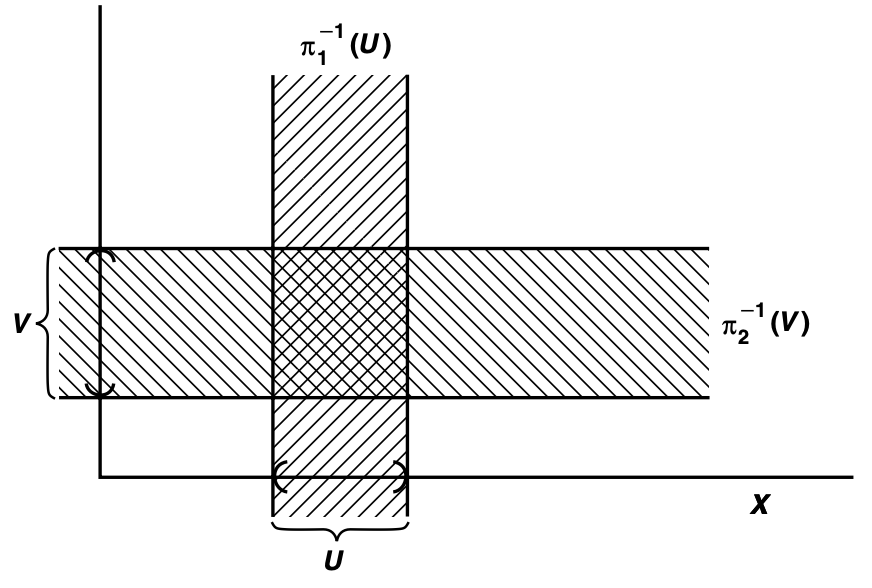
\includegraphics[width=.7\textwidth]{../images/Topology/1.png}
\end{center}

\begin{proof}
Let \(\calt\) denote the product topology on \(X\times Y\); let \(\calt'\) be the topology generated by \(\cals\).
Then \(\calt'\subset \calt\). On the other hand, every basis element \(U\times V\) for the topology \(\calt\) is a
finite intersection of elements of \(\cals\), since
\begin{equation*}
U\times V=\pi_1^{-1}\cap\pi_2^{-1}(V)
\end{equation*}
Hence \(U\times V\in\calt\)
\end{proof}


\subsection{The Subspace Topology}
\label{sec:org8fa9482}
\begin{definition}[]
Let \(X\) be a topological space with topology \(\calt\). If \(Y\subseteq X\), then
\begin{equation*}
\calt_Y=\{Y\cap U\mid U\in\calt\}
\end{equation*}
is a topology on \(Y\), called the \textbf{subspace topology}. With this topology, \(Y\) is called a
\textbf{subspace} of \(X\)
\end{definition}

\begin{lemma}[]
if \(\calb\) is a basis for the topology of \(X\) then the collection
\begin{equation*}
\calb_Y=\{B\cap Y\mid B\in\calb\}
\end{equation*}
is a basis for the subspace topology on \(Y\)
\end{lemma}

\begin{proof}
Given \(U\) open in \(X\) and given \(y\in U\cap Y\), we can choose an element \(B\) of \(\calb\) s.t
. \(y\in B\subset U\). Then \(y\in B\cap Y\subset U\cap Y\). It follows from Lemma \ref{lemma13.2} that \(\calb_Y\) is a
basis for the subspace topology on \(Y\)
\end{proof}

\begin{lemma}[]
Let \(Y\) be a subspace of \(X\). If \(U\) is open in \(Y\) and \(Y\) is open in \(X\),
then \(U\) is open in \(X\)
\end{lemma}

\begin{theorem}[]
if \(A\) is a subspace of \(X\) and \(B\) is a subspace of \(Y\), then the product topology
on \(A\times B\) is the same as the topology \(A\times B\) inherits as a subspace of \(X\times Y\)
\end{theorem}

\begin{proof}
The set \(U\times V\) is the general basis element for \(X\times Y\), where \(U,V\) are open in \(X,Y\)
respectively.  Therefore \((U\times V)\cap(A\times B)\) is the general basis element for the subspace
topology on \(A\times B\). Now
 \begin{equation*}
(U\times V)\cap(A\times B)=(U\cap A)\times (V\cap B)
 \end{equation*}
\end{proof}

Now let \(X\) be an ordered set in the order topology, and let \(Y\) be a subset of \(X\). The
order relation on \(X\), when restricted to \(Y\), makes \(Y\) into an ordered set. However the
resulting order topology on Y need not be the same as the topology that Y inherits as a subspace
of X

\begin{examplle}[]
Consider the subset \(Y=[0,1]\) of the real line \(\R\) in the \emph{subspace} topology. Given \((a,b)\)
\begin{equation*}
(a,b)\cap Y=
\begin{cases}
&(a,b)\\
&[0,b)\\
&(a,1]\\
&Y\text{ or }\emptyset
\end{cases}
\end{equation*}
Sets of the second and third types are not open in the larger space \(\R\)

Note that these sets form a basis for the \emph{order}  topology on \(Y\). Thus we see that in the case
of the set \(Y=[0,1]\) its subspace topology and its order topology are the same
\end{examplle}

Given an ordered set \(X\), a subset \(Y\) of \(X\) is \textbf{convex} in \(X\) if for each pair of
points \(a<b\) of \(Y\), the entire interval \((a,b)\) of points of \(X\) lies in \(Y\). Note
that intervals and rays in \(X\) are convex in \(X\)

\begin{theorem}[]
Let \(X\) be an ordered set in the order topology; let \(Y\) be a subset of \(X\) that is convex
in \(X\). Then the order topology on \(Y\) is the same as the topology \(Y\) inherits as a
subspace of \(X\)
\end{theorem}

\begin{proof}
Consider the ray \((a,+\infty)\) in \(X\). If \(a\in Y\) then
\begin{equation*}
(a,+\infty)\cap Y=\{x\mid x\in Y\text{ and }x>a\}
\end{equation*}
this is an open ray of the ordered set \(Y\). If \(a\not\in Y\), then \(a\) is either a lower bound
on \(Y\) or an upper bound on \(Y\), since \(Y\) is convex. In the former case, \((a,+\infty)\cap Y=Y\);
in the latter case, it is empty

Similarly, \((-\infty,a)\cap Y\) is either an open ray of \(Y\), or \(Y\) itself, or empty. Since the
sets \((a,+\infty)\cap Y\) and \((-\infty,a)\cap Y\) form a subbasis for the subspace topology on \(Y\), and
since each is open in the order topology,and since each is open in the order topology,
the order topology contains the subspace topology

To prove the reverse, note that any open ray of \(Y\) equals the intersection of an open ray
of \(X\) with \(Y\), so it is open in the subspace topology on \(Y\). Since the open rays
of \(Y\) are a subbasis for the order topology, this topology is contained in the subspace topology
\end{proof}

\begin{exercise}
\label{15.1}
Show that if \(Y\) is a subspace of \(X\) and \(A\) is a subset of \(Y\), then the topology \(A\)
inherits as a subspace of \(Y\) is the same as the topology it inherits as a subspace of \(X\)
\end{exercise}

\begin{proof}
For every open set \(U\) of topology of \(X\), \(A\cap(Y\cap U)=A\cap U\).
\end{proof}

\begin{exercise}
\label{ex15.7}
Let \(X\) be an ordered set. If \(Y\) is a proper subset of \(X\) that is convex in \(X\), does
it follow that \(Y\) is an interval or a ray in \(X\)
\end{exercise}

\begin{proof}
Consider \((-\sqrt{2},\sqrt{2})\cap\Q\) which is convex in \(\Q\) but not an interval or a ray
\end{proof}


\subsection{Closed Sets and Limit Points}
\label{sec:org202bab0}
A subset \(A\) of a topological space \(X\) is said to be \textbf{closed} if the set \(X-A\) is open

\begin{theorem}[]
Let \(X\) be a topological space. Then the following conditions hold:
\begin{enumerate}
\item \(\emptyset\) and \(X\) are closed
\item Arbitrary intersection of closed sets are closed
\item Finite unions of closed sets are closed
\end{enumerate}
\end{theorem}

\begin{theorem}[]
\label{thm17.2}
let \(Y\) be a subspace of \(X\). Then a set \(A\) is closed in \(Y\) iff it equals the
intersection of a closed set of \(X\) with \(Y\)
\end{theorem}

\begin{proof}
Assume that \(A=C\cap Y\), where \(C\) is closed in \(X\). Then \(X-C\) is open in \(X\), so
that \((X-C)\cap Y\) is open in \(Y\). But \((X-C)\cap Y=Y-A\). Hence \(Y-A\) is open  in \(Y\)

Assume that \(A\) is closed in \(Y\). Then \(Y-A=U\cap Y\) for some open set \(U\) in \(X\) and \(A=Y\cap(X-U)\)
\end{proof}

\begin{theorem}[]
Let \(Y\) be a subspace of \(X\). If \(A\) is closed in \(Y\) and \(Y\) is closed in \(X\),
then \(A\) is closed in \(X\)
\end{theorem}

Given a subset \(A\) of a topological space \(X\), the \textbf{interior} of \(A\) is defined as the union
of all open sets contained in \(A\), and the \textbf{closure} of \(A\) is defined as the intersection of
all closed sets containing \(A\) (\(\barA\))

\begin{theorem}[]
Let \(Y\) be a subspace of \(X\); let \(A\) be a subset of \(Y\); let \(\barA\) denote the
closure of \(A\) in \(X\). Then the closure of \(A\) in \(Y\) equals \(\barA\cap Y\)
\end{theorem}

\begin{proof}
Let \(B\) denote the closure of \(A\) in \(Y\). The set \(\barA\) is closed in \(X\),
so \(\barA\cap Y\) is closed in \(Y\) by Theorem \ref{thm17.2}. We have \(B\subset(\barA\cap Y)\)

On the other hand, \(B=C\cap Y\) for some \(C\) closed in \(X\). Then \(C\) is a closed set of \(X\)
containing \(A\).
\end{proof}

A set \(A\) \textbf{intersects} a set \(B\) if the intersection \(A\cap B\) is not empty

\begin{theorem}[]
\label{thm17.5}
Let \(A\) be a subset of the topological space \(X\)
\begin{enumerate}
\item \(x\in\barA\) iff every open set \(U\) containing \(x\) intersects \(A\)
\item Suppose the topology of \(X\) is given by a basis, then \(x\in\barA\) iff every basis
element \(b\) containing \(x\) intersects \(A\)
\end{enumerate}
\end{theorem}

\begin{proof}
\begin{enumerate}
\item We consider

\(x\not\in\barA\) iff there exists an open set \(U\) containing \(x\) that does not
intersects \(A\)

If \(x\not\in\barA\), the set \(U=X-\barA\) is an open set containing \(x\) that does not
intersects \(A\), as desired. Conversely, if there exsits an open set \(U\) containing \(x\)
which does not intersects \(A\), then \(X-U\) is a closed set containing \(A\).
Hence \(\barA\subseteq X-U\) and therefore \(x\not\in\barA\)
\end{enumerate}
\end{proof}

\(U\) is an open set containing \(x\) equals \(U\) is a \textbf{neighborhood} of \(x\)

\begin{examplle}[]
Let \(X\) be the real line \(\R\). If \(A=(0,1]\) then \(\barA=[0,1]\) for every neighborhood
of \(0\) intersects \(A\), while every point outside \([0,1]\) has a neighborhood disjoint
from \(A\).

If \(B=\{1/n\mid n\in\Z_+\}\) then \(\barB=\{0\}\cup B\). If \(C=\{0\}\cup(1,2)\) then \(\barC=\{0\}\cup[1,2]\). Also \(\bar{\Q}=\R\).
\end{examplle}

If \(A\)is a subset of the topological space \(X\) and if \(x\) is a point of \(X\), we say
that \(x\) is a \textbf{limit point} of \(A\) if every neighborhood of \(x\) intersects \(A\) in some
point \emph{other than \(x\) itself}. Said differently, \(x\) is a limit point of \(A\) if it belongs to
the closure of \(A-\{x\}\)

\begin{theorem}[]
Let \(A\) be a subset of the topological space \(X\); let \(A'\) be the set of all limit points
of \(A\). Then
\begin{equation*}
\barA=A\cup A'
\end{equation*}
\end{theorem}

\begin{proof}
By Theorem \ref{thm17.5} \(A'\subset\barA\).

Suppose \(x\in\barA-A\). Then \(x\in A'\)
\end{proof}

\begin{corollary}[]
A subset of a topological space is closed iff it contains all its limit points
\end{corollary}

\begin{proof}
\(A\) is closed iff \(\barA=A\)
\end{proof}

In the spaces \(\R\) and \(\R^2\) each one-point set \(\{x_0\}\) is closed since every point different
from \(x_0\) has a neighborhood not intersecting \(\{x_0\}\), so that \(\{x_0\}\) is its own
closure. But this fact is not true for arbitrary topological spaces. Consider the topology on the
three-point set \(\{a,b,c\}\) indicated in Figure \ref{fig:17.3}. The one-point set \(\{b\}\) is not
closed, for its complement is not open

\begin{figure}[htbp]
\centering
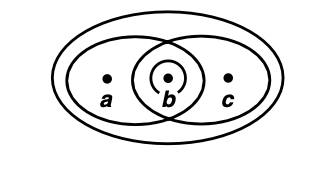
\includegraphics[width=.3\textwidth]{../images/Topology/2.png}
\caption{\label{fig:17.3}we}
\end{figure}

\index{converge}
In an arbitrary topological space, one says that a sequence \(x_1,x_2,\dots\) of points of the
space \(X\) \textbf{converges} to the point \(x\) of \(X\) provided that, corresponding to each
neighborhood \(U\) of \(x\) there is a positive integer \(N\) s.t. \(x_n\in U\) for all \(n\ge N\).
In \(\R\) and \(\R^2\) a sequence cannot converge to more than one point, but in an arbitrary space,
it can. In Figure \ref{fig:17.3} the sequence defined by setting \(x_n=b\) converges not only to
the point \(b\) but also to the point \(a\) and \(c\).

\begin{definition}[]
A topological space \(X\) is called a \textbf{Hausdorff space} if for each pair \(x_1,x_2\) of disjoint
points of \(X\), there exist neighborhoods \(U_1\) and \(U_2\) of \(x_1\) and \(x_2\) respectively,
that are disjoint
\end{definition}

\begin{theorem}[]
Every fintie point set in a Hausdorff space \(X\) is closed.
\end{theorem}

\begin{proof}
It suffices to show that every one-point set \(\{x_0\}\) is closed.
\end{proof}

The condition that finite point sets be closed is in fact weaker than the Hausdorff condition.
For example, the real line \(\R\) in the finite complement topology is not a Hausdorff space, but
it is a space in which finite point sets are closed. The condition that finite point sets be
closed is called the \textbf{\(T_1\) axiom}

\begin{theorem}[]
Let \(X\) be a space satisfying the \(T_1\) axiom; let \(A\) be a subset of \(X\). Then the
point \(x\) is a limit point of \(A\) iff every neighborhood of \(x\) contains infinitely many points
\end{theorem}

\begin{proof}
If \(x\) is a limit point of \(A\) and suppose some neighborhood \(U\) of \(x\) intersects \(A\)
in only finitely many points. Then \(U\) also intersects \(A-\{x\}\) in finitely many points;
let \(\{x_1,\dots,x_m\}\) be the points of \(U\cap(A-\{x\})\). The set \(X-\{x_1,\dots,x_m\}\) is an open set
of \(X\), then
\begin{equation*}
U\cap(X-\{x_1,\dots,x_m\})
\end{equation*}
is a neighborhood of \(x\) that intersects the set \(A-\{x\}\)
\end{proof}

\begin{theorem}[]
If \(X\) is the Hausdorff space, then a sequence of points of \(X\) converges to at most one
point of \(X\)
\end{theorem}

\begin{proof}
Suppose that \(x_n\) is a sequence of points of \(X\) that converges to \(x\). If \(y\neq x\)
let \(U\) and \(V\) be disjoint neighborhoods of \(x\) and \(y\) respectively. Since \(U\)
contains \(x_n\) for all but finitely many values of \(n\), the set \(V\) cannot.
Therefore \(x_n\) cannot converge to \(y\).
\end{proof}

If the sequence \(x_n\) of points of the Hausdorff space \(X\) converges to the point \(x\)
of \(X\), we often write \(x_n\to x\) and we say that \(x\) is the \textbf{limit} of the sequence \(x_n\)

\begin{theorem}[]
Every simply ordered set is a Hausdorff space in the order topology. The product of two Hausdorff
spaces is a Hausdorff space. A subspace of a Hausdorff space is a Hausdorff space.
\end{theorem}

\begin{exercise}
\label{ex17.5}
Let \(X\) be an ordered set in the order topology. Show that \(\ove{(a,b)}\subset[a,b]\). Under what
conditions does equality hold
\end{exercise}

\begin{proof}
It equals the closure iff both endpoints are limit points of the interval, i.e. if \((a,b)\) is not
empty and for every \(x\in(a,b)\) there are \(s,t\in(a,b)\) such that \(a<s<x<t<b\) . This is equivalent to the
requirement that \(a\) has no immediate successor, and \(b\) has no immediate predecessor. Otherwise, if
\(a\) has an immediate successor \(c\) then \((−∞,c)\) is an open set containing \(a\) that does not intersect
\((a,b)\) , and, similarly, if \(b\) has an immediate predecessor \(c\) then \((c,+∞)\) is an open set containing
\(b\) that does not intersect \((a,b)\) .
\end{proof}

\begin{exercise}
\label{ex17.6}
Let \(A\),\(B\) and \(A_\alpha\) denote subsets of a space \(X\). Prove the following
\begin{enumerate}
\item If \(A\subset B\) then \(\barA\subset\barB\)
\item \(\ove{A\cup B}=\barA\cup\barB\)
\item \(\ove{\bigcup A_\alpha}\supset\bigcup\barA_\alpha\); give an example where equality fails
\end{enumerate}
\end{exercise}

\begin{proof}
\begin{enumerate}
\setcounter{enumi}{1}
\item Suppose \(x\not\in\barA\cup\barB\). By Theorem \ref{thm17.5} there is a neighborhoods \(U_A,U_B\)
of \(x\) s.t. \(U_A\cap A=U_B\cap B=\emptyset\).  Let \(U=U_A\cap U_B\). Then \(U\cap(A\cup B)=\emptyset\).
\item Consider \(A_n=(1/n,2]\) for \(n\in\Z_+\)
\end{enumerate}
\end{proof}

\begin{exercise}
\label{ex17.8}
Let \(A\),\(B\) and \(A_\alpha\) denote subsets of a space \(X\). Determine whether the following
equations hold
\begin{enumerate}
\item \(\ove{A\cap B}=\barA\cap\barB\)
\item \(\ove{\bigcap A_\alpha}=\bigcap\barA_\alpha\)
\item \(\ove{A-B}=\barA-\barB\)
\end{enumerate}
\end{exercise}

\begin{proof}
\begin{enumerate}
\item Consider \(A=(1,2)\) and \(B=(0,1)\) in \(\R\). We only have \(\ove{A\cap B}\subset\barA\cap\barB\)
\setcounter{enumi}{2}
\item \(\ove{A-B}\supset\barA-\barB\). \(A=(0,2),B=(0,1)\)
\end{enumerate}
\end{proof}

\begin{exercise}
\label{ex17.13}
\(X\) is Hausdorff iff the \textbf{diagonal} \(\Delta=\{x\times x\mid x\in X\}\) is closed in \(X\times X\).
\end{exercise}

\begin{proof}
\(\Delta\) is closed in \(X\times X\) iff for \(x\neq y\) there is a basis \(x\times y\in U\times V\subset X\times X\)
where  \(U\) and \(V\) are neighborhoods of \(x\) and \(y\) respectively s.t. no
points \((z,z)\in U\times V\)
iff any pair of of different points having disjoint neighborhoods
\end{proof}

\subsection{Continuous Functions}
\label{sec:org81e88d0}
Let \(X\) and \(Y\) be topological spaces. A function \(f:X\to Y\) is said to be \textbf{continuous} if for
each open subset \(V\) of \(Y\) the set \(f^{-1}(V)\) is an open subset of \(X\).

Let's note that if the topology of the range space \(Y\) is given by a basis \(\calb\), then to prove
continuity of \(f\) it suffices to show that the inverse image of every \emph{basis element} is oepn.

If the topology on \(Y\) is given by a subbasis \(\cals\), to prove continuity of \(f\) it will even
suffice to show that the inverse of each \emph{subbasis} element is open.

\begin{examplle}[]
Let's consider a function
\begin{equation*}
f:\R\to\R
\end{equation*}

Now we prove that our definition implies the \(\epsilon\)-\(\delta\) definition

Given \(x_0\in\R\)  and given \(\epsilon>0\) the interval \(V=(f(x_0)-\epsilon,f(x_0)+\epsilon)\) is an open set of the
range space \(\R\). Therefore, \(f^{-1}(V)\) is an open set in the domain space \(\R\).
Because \(x_0\in f^{-1}(V)\), it contains some basis element \((a,b)\) about \(x_0\). We choose
\(\delta\) to be the smaller of the two numbers \(x_0-a\) and \(b-x_0\). Then if \(\abs{x-x_0}<\delta\), the
point \(x\) must be in \((a,b)\), so that \(f(x)\in V\) and \(\abs{f(x)-f(x_0)}<\epsilon\) as desired
\end{examplle}

\begin{examplle}[]
Let \(\R\) denote the set of real numbers in its usual topology. Let
\begin{equation*}
f:\R\to\R_l
\end{equation*}
by the identity function \(f(x)=x\). Then \(f\) is not a continuous function. However
\begin{equation*}
g:\R_l\to\R
\end{equation*}
is continuous
\end{examplle}

\begin{theorem}[]
Let \(X\) and \(Y\) be topological spaces: let \(f:X\to Y\). TFAE
\begin{enumerate}
\item \(f\) is continuous
\item for every \(A\subseteq X\), \(f(\barA)\subset\ove{f(A)}\)
\item for every closed set \(B\) of \(Y\), the set \(f^{-1}(B)\) is closed in \(X\)
\item for each \(x\in X\) and each neighborhood \(V\) of \(f(x)\), there is a neighborhood \(U\)
of \(x\) s.t. \(f(U)\subset V\)
\end{enumerate}


If the condition 4 holds for the point \(x\) of \(X\), we say that \(f\) is \textbf{continuous at the
point \(x\)}
\end{theorem}

\begin{proof}
\(1\to 2\). Assume \(f\) is continuous. Let \(A\subseteq X\) and \(x\in\barA\). Let \(V\) be a neighborhood
of \(f(x)\). Then \(f^{-1}(V)\) is an open set of \(X\) containing \(x\);  it must
intersect \(A\) in some point \(y\). Then \(V\) intersects \(f(A)\) in the point \(f(y)\), so
that \(f(x)\in\ove{f(A)}\)

\(2\to 3\). Let \(B\) be closed in \(Y\) and let \(A=f^{-1}(B)\). We show that \(\barA=A\). We have
\(f(A)=f(f^{-1}(B))\subset B\). Therefore if \(x\in\barA\)
\begin{equation*}
f(x)\in f(\barA)\subset\ove{f(A)}\subset\barB=B
\end{equation*}
so that \(x\inf^{-1}(B)=A\)

\(3\to 1\). easy

\(1\to 4\). easy

\(4\to 1\). not hard \emoji{😊}
\end{proof}

let \(X\) and \(Y\) be topological spaces; let \(f:X\to Y\) be a bijection. If both the
function \(f\) and the inverse function
\begin{equation*}
f^{-1}:Y\to X
\end{equation*}
are continuous, then \(f\) is called a \textbf{homeomorphism}

Suppose that \(f:X\to Y\) is an injective continuous map, where \(X\) and \(Y\) are topological
spaces. Let \(Z\) be the image set \(f(X)\), considered as a subspace of \(Y\); then the
function \(f':X\to Z\) obtained by restricting the range of \(f\)  is bijectiive. If \(f'\) happens
to be a homeomorphism of \(X\) with \(Z\), we say that the map \(f:X\to Y\) is a
\textbf{topological embedding} or simpy an \textbf{embedding} of \(X\) in \(Y\)

\begin{examplle}[]
A bijectiive function \(f:X\to Y\) can be continuous without being a homeomorphism. One such
function is the identity map \(g:\R_l\to\R\)。 Another is the following:

Let \(S^1\) denote the \textbf{unit circle},
\begin{equation*}
S^1=\{x\times y\mid x^2+y^2=1\}
\end{equation*}
considered as a subspace of the plane \(\R^2\) and let
\begin{equation*}
f:[0,1)\to S^1
\end{equation*}
be the map defined by \(f(t)=(\cos 2\pi t,\sin2\pi t)\). \(f\) is continuous but not \(f^{-1}\). The
image under \(f\) of the open set \(U=[0,\frac{1}{4})\) of the domain is not open in \(S^1\), for
the point \(p=f(0)\) lies in no open set \(V\) of \(\R^2\) s.t. \(V\cap S^1\subset f(U)\)

\begin{figure}[htbp]
\centering
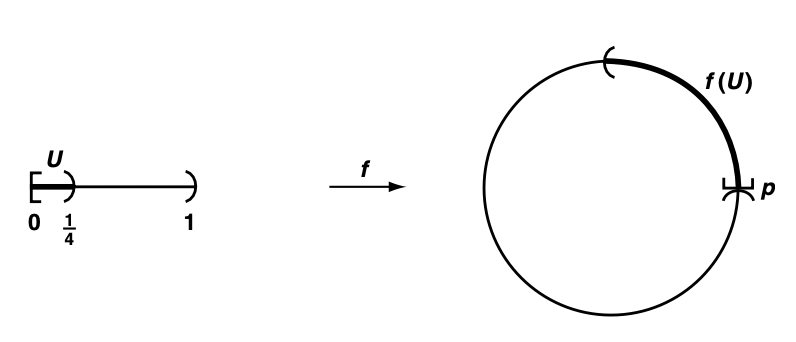
\includegraphics[width=.7\textwidth]{../images/Topology/3.png}
\label{}
\end{figure}
\end{examplle}


\begin{theorem}[Rules for constructing continuous functions]
Let \(X,Y\) and \(Z\) be topological spaces
\begin{enumerate}
\item (Constant function) if \(f:X\to Y\) maps all of \(X\) into the single point \(y_0\) of \(Y\),
then \(f\) is continuous
\item (Inclusion) If \(A\) is a subspace of \(X\), the inclusion function \(j:A\to X\) is continuous
\item (Composites) If \(f:X\to Y\) and \(g:Y\to Z\) are continuous, then the map \(g\circ f:X\to Z\) is continuous
\item (Restricting the domain) if \(f:X\to Y\) is continuous, and if \(A\) is a subspace of \(X\),
then the restricted function \(f|A:A\to Y\) is continuous
\item (Restricting or expanding the range) Let \(f:X\to Y\) be continuous. If \(Z\) is a subspace
of \(Y\) containing the image set \(f(X)\), then the function \(g:X\to Z\) obtained by
restricting the range of \(f\) is continuous. If \(Z\) is a space having \(Y\) as a subspace,
then the function \(h:X\to Z\) obtained by expanding the range of \(f\) is continuous
\item (Local formulation of continuity) The map \(f:X\to Y\) is continuous if \(X\) can be written as
the union of open sets \(U_\alpha\) s.t. \(f|U_\alpha\) is continuous for each \(\alpha\)
\end{enumerate}
\end{theorem}

\begin{proof}
\begin{enumerate}
\item Let \(V\) be open in \(Y\), then \(f^{-1}(V)\) equals \(\emptyset\) or \(X\)
\end{enumerate}
\end{proof}

\begin{theorem}[The pasting lemma]
Let \(X=A\cup B\), where \(A\) and \(B\) are closed in \(X\). Let \(f:A\to Y\) and \(g:B\to Y\) be
continuous. If \(f(x)=g(x)\) for every \(A\cap B\) then \(f\) and \(g\) combine to give a continuous
function \(h:X\to Y\), defined by setting \(h(x)=f(x)\) if \(x\in A\) and \(h(x)=g(x)\) if \(x\in B\)
\end{theorem}

The open set case of the pasting lemma is just the local formulation of continuity

\begin{theorem}[Maps into products]
\label{thm18.4}
Let \(f:A\to X\times Y\) be given by the equation
\begin{equation*}
f(a)=(f_1(a),f_2(a))
\end{equation*}
Then \(f\) is continuous iff the functions
\begin{equation*}
f_1:A\to X \quad\text{ and }\quad f_2:A\to Y
\end{equation*}
are continuous

The maps \(f_1\) and \(f_2\) are called the \textbf{coordinate functions}
\end{theorem}

\begin{proof}
First note that \(\pi_1,\pi_2\) are continuous. For \(\pi_1^{-1}(U)=U\times Y\) and \(\pi_2^{-1}(V)=X\times V\) and
these sets are open if \(U\) and \(V\) are open. Note that for each \(a\in A\)
\begin{equation*}
f_1(a)=\pi_1(f(a))\quad\text{ and }\quad f_2(a)=\pi_2(f(a))
\end{equation*}
If \(f\) is continuous, then \(f_1,f_2\) are continuous

Conversely, we show that for each basis element \(U\times V\) for the topology \(X\times Y\) its inverse
image \(f^{-1}(U\times V)\) is open. \(a\in f^{-1}(U\times V)\) iff \(f(a)\in(U\times V)\) iff \(f_1(a)\in U\)
and \(f_2(a)\in V\). Therefore
\begin{equation*}
f^{-1}(U\times V)=f_1^{-1}(U)\times f_2^{-1}(V)
\end{equation*}
\end{proof}

\begin{exercise}
\label{ex18.11}
Let \(F:X\times Y\to Z\). We say that \(F\) is \textbf{continuous in each variable separately} if for
each \(y_0\) in \(Y\), the map \(h:X\to Z\) defined by \(h(x)=F(x\times y_0)\) is continuous, and for
each \(x_0\) in \(X\), the map \(k:Y\to Z\) defined by \(k(y)=F(x_0\times y)\) is continuous. Show that
if \(F\) is continuous, then \(F\) is continuous in each variable separately.
\end{exercise}

\begin{exercise}
\label{ex18.12}
Let \(F:\R\times \R\to\R\) be defined by the equation
\begin{equation*}
F(x\times y)=
\begin{cases}
xy/(x^2+y^2)&\text{if }x\times y\neq 0\times 0\\
0
\end{cases}
\end{equation*}
\begin{enumerate}
\item Show that \(F\) is continuous in each variable separately
\item Compute the function \(g:\R\to\R\) defined by \(g(x)=F(x\times x)\)
\item Show that \(F\) is not continuous
\end{enumerate}
\end{exercise}

\subsection{The Product Topology}
\label{sec:org9552938}

\begin{definition}[]
Let \(J\) be an index set. Given a set \(X\), we define \textbf{\(J\)-tuple} of elements of \(X\) to be a
function \(\bx:J\to X\). If \(\alpha\) is an element of \(j\), we often denote the value of \(\bx\) at \(\alpha\)
by \(x_\alpha\); we call it the \(\alpha\)th \textbf{coordinate} of \(\bx\). And we often denote the function \(\bx\)
itself by the symbol
\begin{equation*}
(x_\alpha)_{\alpha\in J}
\end{equation*}
We denote the set of all \(J\)-tuples of elements of \(X\) by \(X^J\)
\end{definition}

\begin{definition}[]
Let \(\{A_\alpha\}_{\alpha\in J}\) be an indexed family of sets; let \(X=\bigcup_{\alpha\in J}A_\alpha\). The \textbf{cartesian product}
of this indexed family, denoted by
\begin{equation*}
\prod_{\alpha\in J}A_\alpha
\end{equation*}
is defined to be the set of all \(J\)-tuples \((x_\alpha)_{\alpha\in J}\) of elements of \(X\)
s.t. \(x_\alpha\in A_\alpha\)  for each \(\alpha\in J\). That is, it is the set of all functions
\begin{equation*}
\bx:J\to\bigcup_{\alpha\in J}A_\alpha
\end{equation*}
s.t. \(\bx(\alpha)\in A_\alpha\) for each \(\alpha\in J\)
\end{definition}

\begin{definition}[]
Let \(\{X_\alpha\}_{\alpha\in J}\) be an indexed family of topological spaces. Let us take as a basis for a
topology on the product space
\begin{equation*}
\prod_{\alpha\in J}X_\alpha
\end{equation*}
the collection of all sets of the form
\begin{equation*}
\prod_{\alpha\in J}U_\alpha
\end{equation*}
where \(U_\alpha\) is open in \(X_\alpha\), for each \(\alpha\in J\). The topology generated by this basis is
called the \textbf{box topology}
\end{definition}

Now we generalize the subbasis formulation of the definition. Let
\begin{equation*}
\pi_\beta:\prod_{\alpha\in J}X_\alpha\to X_\beta
\end{equation*}
be the function assigning to each element of the product space its \(\beta\)th coordinate
\begin{equation*}
\pi_\beta((x_\alpha)_{\alpha\in J})=x_\beta
\end{equation*}
it is called the \textbf{projection mapping} associated with the index \(\beta\)

\begin{definition}[]
Let \(\cals_\beta\) denote the collection
\begin{equation*}
\cals_\beta=\{\pi_\beta^{-1}(U_\beta)\mid U_\beta\text{ open in }X_\beta\}
\end{equation*}
and let \(\cals\) denote the union of these collections
\begin{equation*}
\cals=\bigcup_{\beta\in J}\cals_\beta
\end{equation*}
The topology generated by the subbasis \(\cals\)  is called the \textbf{product topology}. In this
topology \(\prod_{\alpha\in J}X_\alpha\) is called a \textbf{product space}
\end{definition}

To compare these topologies, we consider the basis \(\calb\) that \(\cals\) generates. The
collection \(\calb\) consists of all finite intersections of elements of \(\cals\). If we intersect
elements belonging to the same one of the sets \(\cals_\beta\) we do not get anything new, because
\begin{equation*}
\pi_\beta^{-1}(U_\beta)\cap\pi_\beta^{-1}(V_\beta)=\pi_\beta^{-1}(U_\beta\cap V_\beta)
\end{equation*}
We get something new only when we intersect elements from different sets \(\cals_\beta\). Thus the typical
element of the basis \(\calb\) can be described as follows: let \(\beta_1,\dots,\beta_n\) be a finite set of
distinct indices from the index set \(J\), and let \(U_{\beta_i}\) be an open set in \(X_{\beta_i}\)
for \(i=1,\dots,n\). Then
\begin{equation*}
B=\pi_{\beta_1}^{-1}(U_{\beta_1})\cap\dots\cap\pi_{\beta_n}^{-1}(U_{\beta_n})
\end{equation*}
is the typical element of \(\calb\)

Now a point \(\bx=(x_\alpha)\) is in \(B\) iff its \(\beta_1\)th coordinate is in \(U_{\beta_1}\),  its \(\beta_2\)th
coordinate is in \(U_{\beta_2}\), and so on. As a result, we can write \(B\) as the product
\begin{equation*}
B=\prod_{\alpha\in J}U_\alpha
\end{equation*}
where \(U_\alpha\) denotes the entire space \(X_\alpha\) if \(\alpha\neq\beta_1,\dots,\beta_n\)

\begin{theorem}[Comparison of the box and product topologies]
The box topology on \(\prod X_\alpha\) has as basis all sets of the form \(\prod U_\alpha\), where \(U_\alpha\) is open
in \(X_\alpha\) for each \(\alpha\). The product topology on \(\prod X_\alpha\) has as basis all sets of the
form \(U_\alpha\), where \(U_\alpha\) is open in \(U_\alpha\) for  each \(\alpha\) and \(U_\alpha\) equals \(X_\alpha\) except
for finitely many values of \(\alpha\)
\end{theorem}

\begin{quoting}
Whenever we consider the product \(X_\alpha\), we shall assume it is given the product topology unless
we specifically state otherwise.
\end{quoting}

\begin{theorem}[]
\label{thm19.2}
Suppose the topology on each space \(X_\alpha\) is given by a basis \(\calb_\alpha\). The collection of all
sets of the form
\begin{equation*}
\prod_{\alpha\in J}B_\alpha
\end{equation*}
where \(B_\alpha\in \calb_\alpha\) for each \(\alpha\), will serve as a basis for the box topology on \(\prod_{\alpha\in J}X_\alpha\)

The collection of all sets of the same form, where \(B_\alpha\in\calb_\alpha\) for finitely many indices \(\alpha\)
and \(B_\alpha=X_\alpha\) for all the remaining indices, will serve as a basis for the product
topology \(\prod_{\alpha\in J}X_\alpha\)
\end{theorem}

\begin{theorem}[]
\label{thm19.3}
Let \(A_\alpha\) be a subspace of \(X_\alpha\) for each \(\alpha\in J\). Then \(\prod A_\alpha\) is a subspace of \(\prod X_\alpha\)
is both products are given the box topology or product topology
\end{theorem}

\begin{theorem}[]
\label{thm19.4}
If each space \(X_\alpha\) is a Hausdorff space, then \(\prod X_\alpha\) is a Hausdorff space in both the box
and product topologies
\end{theorem}

\begin{theorem}[]
\label{thm19.5}
Let \(\{X_\alpha\}\) be an indexed family of spaces; let \(A_\alpha\subseteq X_\alpha\)  for each \(\alpha\). If \(\prod X_\alpha\) is given
either the product or the box topology, then
\begin{equation*}
\prod \barA_\alpha=\ove{\prod A_\alpha}
\end{equation*}
\end{theorem}

\begin{proof}
Let \(\bx=(x_\alpha)\) be a point of \(\prod\barA_\alpha\); we show that \(\bx\in\ove{\prod A_\alpha}\). Let \(U=\prod U_\alpha\)  be a
basis element for either the box or product topology that contains \(\bx\). Since \(x_\alpha\in\barA_\alpha\),
we can choose a point \(y_\alpha\in U_\alpha\cap A_\alpha\). Then \(\by=(y_\alpha)\) belongs to both \(U\) and \(\prod A_\alpha\).
Since \(U\) is arbitrary, it follows that \(\bx\in\prod A_\alpha\)

Conversely, suppose \(\bx=(x_\alpha)\) lies in the closure of \(\prod A_\alpha\), in either topology. We show
that for any given index \(\beta\), we have \(x_\beta\in\barA_\beta\). Let \(V_\beta\) be an arbitrary open set of \(X_\beta\)
containing \(x_\beta\). Since \(\pi_\beta^{-1}(V_\beta)\) is open in \(\prod X_\alpha\) in either topology, it contains a
point \(\by=(y_\alpha)\) of \(\prod A_\alpha\). Then \(y_\beta\) belongs to \(V_\beta\cap A_\beta\). It follows that \(x_\beta\in\barA_\beta\)
\end{proof}

\begin{theorem}[]
\label{thm19.6}
Let \(f:A\to\prod_{\alpha\in J}X_\alpha\) be given by the equation
\begin{equation*}
f(a)=(f_\alpha(a))_{\alpha\in J}
\end{equation*}
where \(f_\alpha:A\to X_\alpha\) for each \(\alpha\). Let \(\prod X_\alpha\) have the product topology. Then the function \(f\)
is continuous iff each function \(f_\alpha\) is continuous
\end{theorem}

\begin{proof}
\(\Rightarrow\) composition of continuous functions is continuous

\(\Leftarrow\) Suppose that each coordinate function \(f_\alpha\) is continuous. To prove that \(f\) is
continuous, it suffices to prove that the inverse image under \(f\) of each subbasis element is
open in \(A\).  A typical subbasis element for the
product topology on \(\prod X_\alpha\) is a set of the form \(\pi_\beta^{-1}(U_\beta)\) where \(\beta\) is some index
and \(U_\beta\) is open in \(X_\beta\). now
\begin{equation*}
f^{-1}(\pi_\beta^{-1}(U_\beta))=f_\beta^{-1}(U_\beta)
\end{equation*}
because \(f_\beta=\pi_\beta\circ f\). Since \(f_\beta\) is continuous, this set is open in \(A\)
\end{proof}

\begin{examplle}[]
Consider \(\R^\omega\) and define \(f:\R\to\R^\omega\)
\begin{equation*}
f(t)=(t,t,\dots)
\end{equation*}
\(f\) is continuous if \(\R^\omega\) is given the box topology. Consider the basis element
\begin{equation*}
B=(-1,1)\times(-\frac{1}{2},\frac{1}{2})\times(-\frac{1}{3},\frac{1}{3})\times\dots
\end{equation*}
We assert that \(f^{-1}(B)\) is not open in \(\R\). \(f^{-1}(B)=\{0\}\)
\end{examplle}

\begin{exercise}
\label{ex19.6}
let \(\bx_1,\bx_2,\dots\) be a sequence of the points of the products space \(\prod X_\alpha\). Show that this
sequence converges to the point \(\bx\) iff the sequence \(\pi_\alpha(\bx_1),\pi_\alpha(\bx_2),\dots\) converges
to \(\pi_\alpha(\bx)\) for each \(\alpha\)
\end{exercise}

\begin{proof}
Given a neighborhood \(U=\prod U_\alpha\) of \(\bx\), for each \(\alpha\), we have \(N_\alpha\) s.t. \(\pi_\alpha(x_n)\in U_\alpha\) for
all \(n\ge N_\alpha\). If \(U_\alpha=X_\alpha\) we take \(N_\alpha=1\). Hence in product topology we have only finitely
many \(N_\alpha>1\) and we can take max. This fails in box topology as it might not have max
\end{proof}

\begin{exercise}
\label{ex19.7}
Let \(\R^\infty\) be the subset of \(\R^\omega\) consisting of all sequences that are ``eventually zero'', that
is, all sequences \((x_1,x_2,\dots)\) s.t. \(x_i\neq0\) for only finitely many values of \(i\). What is
the closure of \(\R^\infty\) in \(\R^\omega\) in the box and product topologies? justify your answer
\end{exercise}

\begin{proof}


If \(\R^\infty\) is given the product topology, given a point \(\bx\in\R^\omega\) and a neighborhood \(U=\bigcup_i U_i\)
where \(U_i\) is a proper open subset of \(\R\) for finitely many \(i\in\omega\). Choose \(y_i\in U_i\)
and \(y_j=0\) if \(U_j=\R\). Then \(\by\in\R^\infty\cap U\). Hence \(x\in\ove{\R^\infty}\)

For box topology, \(\ove{\R^{\infty}}=\R^\infty\).
\end{proof}

\begin{exercise}
Given sequences \((a_1,a_2,\dots)\) and \((b_1,b_2,\dots)\) of real numbers with \(a_i>0\) for all \(i\),
define \(h:\R^\omega\to\R^\omega\) by the equation
\begin{equation*}
h((x_1,x_2,\dots))=(a_1x_1+b_1,a_2x_2+b_2,\dots)
\end{equation*}
Show that if \(\R^\omega\) is given the product topology, \(h\) is a homeomorphism of \(\R^\omega\) with
itself. What happens if \(\R^\omega\) is given the box topology
\end{exercise}

\begin{proof}
both box and product
\end{proof}


\subsection{The Metric Topology}
\label{sec:org069fb1b}
\begin{definition}[]
A \textbf{metric} on a set \(X\) is a function
\begin{equation*}
d:X\times X\to R
\end{equation*}
having the following properties
\begin{enumerate}
\item \(d(x,y)\ge0\) for all \(x,y\in X\); equality holds iff \(x=y\)
\item \(d(x,y)=d(y,x)\) for all \(x,y\in X\)
\item \(d(x,y)+d(y,z)\ge d(x,z)\) for all \(x,y,z\in X\)
\end{enumerate}
\end{definition}

Given a metric \(d\) on \(X\), the number \(d(x,y)\) is often called the \textbf{distance} between \(x\)
and \(y\) in the metric \(d\). Given \(\epsilon>0\) consider the set
\begin{equation*}
B_d(x,\epsilon)=\{y\mid d(x,y)<\epsilon\}
\end{equation*}
of all points \(y\) whose distance from \(x\) is less than \(\epsilon\). It is called the \textbf{\(\epsilon\)-ball
centered at \(x\)}

\begin{definition}[]
If \(d\) is a metric on the set \(X\), then the collection of all \(\epsilon\)-balls \(B_d(x,\epsilon)\)
for \(x\in X\) and \(\epsilon>0\) is a basis for a topology on \(X\), called the \textbf{metric topology} induced
by \(d\)
\end{definition}

Check the second condition.

If \(y\in B(x,\epsilon)\) then there is a basis element \(B(y,\delta)\) \emph{centered} at \(y\) that is contained
in \(B(x,\epsilon)\). Define \(\delta\) to be \(\epsilon-d(x,y)\). Then \(B(y,\delta)\subset B(x,\epsilon)\), for if \(z\in B(y,\delta)\)
then \(d(y,z)<\epsilon-d(x,y)\), from which we conclude that
\begin{equation*}
d(x,z)\le d(x,y)+d(y,z)<\epsilon
\end{equation*}

\begin{figure}[htbp]
\centering
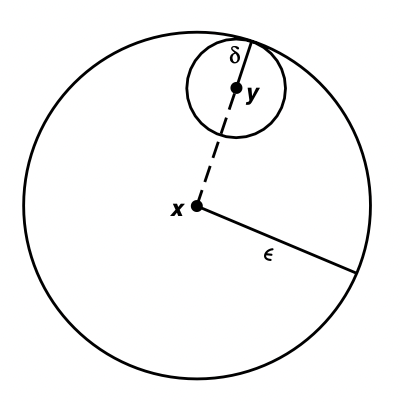
\includegraphics[width=.4\textwidth]{../images/Topology/4.png}
\label{}
\end{figure}

Let \(B_1\) and \(B_2\) be two basis element and let \(y\in B_1\cap B_2\).We have just shown that we can
choose positive numbers \(\delta_1\) and \(\delta_2\) so that \(B(y,\delta_1)\subset B_1\) and \(B(y,\delta_2)\subset B_2\).
Let \(\delta=\min\{\delta_1,\delta_2\}\) we conclude \(B(y,\delta)\subset B_1\cap B_2\). Hence
\begin{quoting}
A set \(U\) is open in the metric topology induced by \(d\) iff for each \(y\in U\) there is
a \(\delta>0\) s.t. \(B_d(y,\delta)\subset U\)
\end{quoting}

\begin{definition}[]
If \(X\) is a topological space, \(X\) is said to be \textbf{metrizable} if there exists a metric \(d\) on
the set \(X\) that induces the topology of \(X\).  A \textbf{metric space} is a metrizable space together
with a specific metric \(d\) that gives the topology of \(X\)
\end{definition}

\begin{definition}[]
Let \(X\) be a metric space with metric \(d\). A subset \(A\) of \(X\) is said to be \textbf{bounded} if
there is some number \(M\) s.t.
\begin{equation*}
d(a_1,a_2)\le M
\end{equation*}
for every pair \(a_1,a_2\) of points of \(A\). If \(A\) is bounded and nonempty, the \textbf{diameter}
of \(A\) is defined to be the number
\begin{equation*}
\diam A=\sup\{d(a_1,a_2)\mid a_1,a_2\in A\}
\end{equation*}
\end{definition}

\begin{theorem}[]
Let \(X\) be a metric space with metric \(d\). Define \(\bard:X\times X\to\R\) by the equation
\begin{equation*}
\bard(x,y)=\min\{d(x,y),1\}
\end{equation*}
Then \(\bard\) is a metric that induces the same topology as \(d\).
\end{theorem}

The metric \(\bard\) is called the \textbf{standard bounded metric} corresponding to \(d\).

\begin{proof}
Check
\begin{equation*}
\bard(x,z)\le\bard(x,y)+\bard(y,z)
\end{equation*}
If both \(d(x,y)\) and \(d(y,z)\) are <1. Then
\begin{equation*}
d(x,z)\le d(x,y)+d(y,z)=\bard(x,y)+\bard(y,z)
\end{equation*}

Note that in any metric space, the collection of \(\epsilon\)-balls with \(\epsilon<1\) forms a basis for the
metric topology
\end{proof}

\begin{definition}[]
Given \(\bx=(x_1,\dots,x_n)\) in \(\R^n\), we define the \textbf{norm} of \(\bx\) by
\begin{equation*}
\norm{x}=\sqrt{x_1^2+\dots+x_n^2}
\end{equation*}
and we define the \textbf{euclidean metric} \(d\) on \(\R^n\) by
\begin{equation*}
d(\bx,\by)=\norm{\bx-\by}=\sqrt{(x_1-y_1)^2+\dots+(x_n-y_n)^2}
\end{equation*}
We define the \textbf{square metric} \(\rho\) by
\begin{equation*}
\rho(\bx,\by)=\max\{\abs{x_1-y_1},\dots,\abs{x_y,y_n}\}
\end{equation*}
\end{definition}

Check the third condition for \(\rho\). for each \(i\in\N_+\)
\begin{equation*}
\abs{x_i-z_i}\le\abs{x_i-y_i}+\abs{y_i-z_i}
\end{equation*}
then
\begin{equation*}
\abs{x_i-z_i}\le\rho(\bx,\by)+\rho(\by,\bz)
\end{equation*}

On the real line \(\R\), these two metrics coincide with the standard metric for \(\R\)

\begin{lemma}[]
Let \(d\) and \(d'\) be two metrics on the set \(X\); let \(\calt\) and \(\calt'\) be the topologies they
induce, respectively. Then \(\calt'\) is finer than \(\calt\) iff for each \(x\in X\) and each \(\epsilon>0\)
there exists a \(\delta>0\) s.t.
\begin{equation*}
B_{d'}(x,\delta)\subset B_d(x,\epsilon)
\end{equation*}
\end{lemma}

\begin{theorem}[]
The topologies on \(\R^n\) induced by the euclidean metric \(d\) and the square metric \(\rho\) are the
same as the product topology on \(\R^n\)
\end{theorem}

\begin{proof}
Let \(\bx=(x_1,\dots,x_n)\) and \(\by=(y_1,\dots,y_n)\) be two points of \(\R^n\). We have
\begin{equation*}
\rho(\bx,\by)\le d(\bx,\by)\le\sqrt{n}\rho(\bx,\by)
\end{equation*}
The first inequality shows that
\begin{equation*}
B_d(\bx,\epsilon)\subset B_\rho(\bx,\epsilon)
\end{equation*}
for all \(\bx\) and \(\epsilon\). Similarly
\begin{equation*}
B_\rho(\bx,\epsilon/\sqrt{n})\subset B_d(\bx,\epsilon)
\end{equation*}
It follows from the preceding lemma that the two metric topologies are the same

Next we show that the product topology is the same as that given by the metric \(\rho\). First let
\begin{equation*}
B=(a_1,b_1)\times\dots\times(a_n,b_n)
\end{equation*}
be a basis element for the product topology, and let \(\bx=(x_1,\dots,x_n)\in B\). For each \(i\) there is
an \(\epsilon_i\) s.t.
\begin{equation*}
(x_i-\epsilon_i,x_i+\epsilon_i)\subset (a_i,b_i)
\end{equation*}
choose \(\epsilon=\min\{\epsilon_1,\dots,\epsilon_n\}\). Then \(B_\rho(\bx,\epsilon)\subset B\).
\end{proof}

Now we consider the infinite cartesian product \(\R^\omega\). It is natural to try to generalize the
metrics \(d\) and ρ to this space. For instance, one can attempt to define a metric \(d\)
on \(\R^\omega\) by the equation

\begin{equation*}
d(x,y)=\sqrt{\sum_{i=1}^\infty(x_i-y_i)^2}
\end{equation*}
But this equation does not always make sense, for the series in question need not converge. (This
equation does define a metric on a certain important subset of \(\R^\omega\), however; see the
exercises.)

Similarly, one can attempt to generalize the square metric ρ to \(\R^\omega\) by defining
\begin{equation*}
\rho(x,y)=\sup\{\abs{x_n-y_n}\}
\end{equation*}
Again, this formula does not always make sense. If however we replace the usual
metric \(d(x,y)=\abs{x-y}\) on \(\R\) by its bounded counterpart \(\bard(x,y)=\min\{\abs{x-y},1\}\), then
this definition does make sense; it gives a metric on \(\R^\omega\) called the \emph{uniform metric}

\index{uniform metric}
\index{uniform topology}
\begin{definition}[]
Given an index set \(J\), and given points \(\bx=(x_\alpha)_{\alpha\in J}\) of \(\R^J\), let's define a
metric \(\barrho\) on \(\R^J\) by
\begin{equation*}
\barrho(\bx,\by)=\sup\{\bard(x_\alpha,y_\alpha)\mid\alpha\in J\}
\end{equation*}
where \(\bard\) is the standard bounded metric on \(\R\). It is easy to check that \(\barrho\) is
indeed a metric; it is called the \textbf{uniform metric} on \(\R^J\), and the topology it induces is called
the \textbf{uniform topology}
\end{definition}

\begin{theorem}[]
The uniform topology on \(\R^J\) is finer than the product topology and coarser than the box
topology; these three topologies are all different is \(J\) is infinite
\end{theorem}

\begin{proof}
Suppose that we are given a point \(\bx=(x_\alpha)_{\alpha\in J}\) and a product topology basis
element \(\prod U_\alpha\). Let \(\alpha_1,\dots,\alpha_n\) be the indices for which \(U_\alpha\neq\R\). Then for each \(i\),
choose \(\epsilon_i>0\) so that \(B_{\bard}(x_{\alpha_i},\epsilon_i)\subset U_{\alpha_i}\). Let \(\epsilon=\min\{\epsilon_1,\dots,\epsilon_n\}\), then
\(B_{\bard}(\bx,\epsilon)\subset\prod U_\alpha\).
\end{proof}

\begin{theorem}[]
Let \(\bard(a,b)=\min\{\abs{a-b},1\}\) be the standard bounded metric on \(\R\). If \(\bx,\by\in\R^\omega\),
define
\begin{equation*}
D(\bx,\by)=\sup\left\{
\frac{\bard(x_i,y_i)}{i}
\right\}
\end{equation*}
Then \(D\) is a metric that induces the product topology on \(\R^\omega\)
\end{theorem}

\begin{proof}
First let \(U\) be open in the metric topology and let \(\bx\in U\); Choose an
\(\epsilon\)-ball \(B_D(\bx,\epsilon)\subset U\). Then choose \(N\) large enough that \(1/N<\epsilon\). Let \(V\) be the basis
element for the product topology
\begin{equation*}
V=(x_1-\epsilon,x_1+\epsilon)\times\dots\times(x_N-\epsilon,x_N+\epsilon)\times\R\times\R\times\dots
\end{equation*}
We assert that \(V\subset B_D(\bx,\epsilon)\). Given any \(\by\in\R^\omega\)
\begin{equation*}
\frac{\bard(x_i,y_i)}{i}\le\frac{1}{N}\hspace{1cm}\text{for }i\ge N
\end{equation*}
therefore
\begin{equation*}
D(\bx,\by)\le\max\left\{\frac{\bard(x_1,y_1)}{1},\dots,\frac{\bard(x_N,y_N)}{N},\frac{1}{N}\right\}
\end{equation*}
If \(\by\in V\) then \(D(\bx,\by)<\epsilon\), so that \(V\subset B_D(\bx,\epsilon)\)

Conversely, consider a basis element
\begin{equation*}
U=\prod_{i\in\Z_+}U_i
\end{equation*}
for the product topology, where \(U_i\) is open in \(\R\) in \(\R\) for \(i= \alpha_1,\dots,\alpha_n\) and \(U_i=\R\)
for all other indices. Given \(\bx\in U\), consider an interval \((x_i-\epsilon_i,x_i+\epsilon_i)\subset U_i\)
for \(i= \alpha_1,\dots,\alpha_n\); choose each \(\epsilon_i\le 1\), then define
\begin{equation*}
\epsilon=\min\{\epsilon/i\mid i= \alpha_1,\dots,\alpha_n\}
\end{equation*}
we assert that
\begin{equation*}
\bx\in B_D(\bx,\epsilon)\subset U
\end{equation*}
let \(\by\) be a point of \(B_D(\bx,\epsilon)\). then for all \(i\)
\begin{equation*}
\frac{\bard(x_i,y_i)}{i}\le D(\bx,\by)<\epsilon
\end{equation*}
Now if \(i= \alpha_1,\dots,\alpha_n\) then \(\epsilon\le\epsilon_i/i\) so that \(\bard(x_i,y_i)<\epsilon_i\le 1\). It follows
that \(\abs{x_i-y_i}<\epsilon_i\). Therefore \(\by\in\prod U_i\)
\end{proof}

\begin{exercise}
Let \(X\) be a metric space with metric \(d\)
\begin{enumerate}
\item \(d:X\times X\to\R\) is continuous
\item Let \(X'\) denote a space having the same underlying set as \(X\). Show that if \(d:X'\times X'\to\R\)
is continuous, then the topology of \(X'\) is finer than the topology of \(X\)
\end{enumerate}
\end{exercise}

\begin{proof}
\begin{enumerate}
\item Prove that for any \(U\) open in \(\R\) and \((x,y)\in d^{-1}(U)\) there is a basis element \(B\)
of \(X\times X\) s.t. \((x,y)\in B\subset d^{-1}(U)\). Suppose \(d(x,y)=a\). There is a \(\epsilon\)
s.t. \((a-\epsilon,a+\epsilon)\subset U\). We take \(B=B_d(x,\epsilon/2)\times B_d(y,\epsilon/2)\). for
any \((x,y)\in B\), \(d(x,y)\in(a-\epsilon,a+\epsilon)\)
\item for every fixed \(x\in X'\), \(d_x(y):X'\to\R,y\mapsto d(x,y)\) is continuous. Therefore every
\(B_d(x,r)=d_x^{-1}((-\infty,r))\) must be open in \(X'\)
\end{enumerate}
\end{proof}

\begin{exercise}
\label{ex20.4}
Consider the product, uniform and box topologies on \(\R^\omega\)
\begin{enumerate}
\item in which topologies are the following functions from \(\R\) to \(\R^\omega\) continuous
\begin{align*}
&f(t)=(t,2t,3t,\dots)\\
&g(t)=(t,t,t,\dots)\\
&h(t)=(t,\frac{1}{2}t,\frac{1}{3}t,\dots)
\end{align*}
\item in which topologies do the following sequences converge
\begin{alignat*}{2}
&\bw_1=(1,1,1,1,\dots)&&\bx_1=(1,1,1,1,\dots)\\
&\bw_2=(0,2,2,2,\dots)&&\bx_2=(0,\frac{1}{2},\frac{1}{2},\frac{1}{2},\dots)\\
&\bw_3=(0,0,3,3,\dots)\quad&&\bx_3=(0,0,\frac{1}{3},\frac{1}{3})\\
&\quad\dots&&\quad\dots\\
&\by_1=(1,0,0,0,\dots)&&\bz_1=(1,1,0,0,\dots)\\
&\by_2=(\frac{1}{2},\frac{1}{2},0,0,\dots)&&\bz_2=(\frac{1}{2},\frac{1}{2},0,0,\dots)\\
&\by_3=(\frac{1}{3},\frac{1}{3},\frac{1}{3},0,\dots)&&\bz_3=(\frac{1}{3},\frac{1}{3},0,0,\dots)
\end{alignat*}
\end{enumerate}
\end{exercise}

\begin{proof}
\begin{enumerate}
\item For box topology, consider open set
\begin{equation*}
B=(-1,1)\times(-\frac{1}{2},\frac{1}{2})\times(-\frac{1}{3},\frac{1}{3})\times\dots
\end{equation*}
\(f^{-1}(B)=g^{-1}(B)=h^{-1}(B)=\{0\}\) which is not open.

For uniform topology. First, \(f^{-1}(B_{\barrho}(\textbf{0},1))\subset f^{-1}(\prod_{n\in\Z_+}(-1,1))=\{0\}\). At the
same time, for \(k(t)=(a_1t,a_2t,\dots)\) equals \(g\) or \(h\)
and \(k(t)\in B_{\barrho}(\bx,\epsilon)\), then for
every \(n\in\Z_+\),  \(\abs{x_n-a_nt}\le\sup_{n\in\Z_+}\abs{x_n-a_nt}=\delta<\epsilon\).
And
for \(\abs{z}<\frac{\epsilon-\delta}{2}\)
\end{enumerate}
\begin{equation*}
\abs{x_n-a_n(t+z)}\le\abs{x_n-a_nt}+a_n\abs{z}<\delta+\frac{\epsilon-\delta}{2}=\frac{\epsilon+\delta}{2}<\epsilon
\end{equation*}
Hence \(k((t-\frac{\epsilon-\delta}{2},t+\frac{\epsilon-\delta}{2}))\subset B_{\barrho}(\bx,\epsilon)\) and \(k^{-1}(B_{\barrho}(\bx,\epsilon))\)
is open.

Product topology. all three
\begin{enumerate}
\setcounter{enumi}{1}
\item If a sequence converges to a point, and we change the topology to a coarser one, then
the sequence still converges to the point. Therefore for each sequence we may specify the
finest topology out of the three given topologies in which it converges to some point.

For \(\{\bw_n\}\) it is the product topology, for  \(\{\bx_n\}\) and \(\{y_n\}\)  it is the uniform
topology and for \(\{\bz_n\}\) it is the product topology

\(\{\bx_n\}\) converges to \(\textbf{0}\) in the uniform topology, as
for \(n>\frac{1}{\epsilon}\), \(\bx_n\in B_{\barrho}(\textbf{0},\epsilon)\)
\end{enumerate}
\end{proof}

\begin{exercise}
\label{ex20.5}
Let \(\R^\infty\) be the subset of \(\R^\omega\) consisting of all sequences that are eventually zero. What
is the closure of \(\R^\infty\) in \(\R^\omega\) in the uniform topology
\end{exercise}

\begin{proof}
Let \(X\in\R^\omega\) be the set of all sequences of real numbers that converge to 0 in \(\R\). Note
that \(\R^\infty\subset X\). If \(\by\not\in X\), then there is \(\epsilon>0\) s.t. for every \(k\in\Z_+\) there
is \(n_k\ge k\) s.t. \(\abs{y_{n_k}}\ge\epsilon\). Hence if \(\bz\in B_{\barrho}(\by,\frac{\epsilon}{2})\), for
every \(k\in\Z_+\), \(\abs{z_{n_k}}>\abs{y_{n_k}}-\frac{\epsilon}{2}\ge\frac{\epsilon}{2}\)
and \(B_{\barrho}(\by,\frac{\epsilon}{2})\) doesn't contain any points of \(X\). Therefore \(X\) is closed
and contains the closure of \(\R^\infty\).

At the same time, for every \(\bx\in X\) and \(\epsilon>0\) there is \(N\in\Z_+\) s.t.
for \(n\ge N\), \(\abs{x_n}<\frac{\epsilon}{2}\) and \(\by=(x_1,\dots,x_N,0,0,\dots)\in B_{\barrho(\bx,\epsilon)}\cap\R^\infty\).
\end{proof}

\subsection{The Metric Topology (continued)}
\label{sec:org947e0fc}
\emph{subspaces} of metric spaces behave the way one would wish them to; if \(A\) is a subspace of the
topological space \(X\) and \(d\) is a metric for \(X\), then the restriction of \(d\)
to \(A\times A\) is a metric for the topology of \(A\)

The \emph{Hausdorff axiom} is satisfied by every metric topology

\begin{theorem}[]
Let \(f:X\to Y\); let \(X\) and \(Y\) be metrizable with metrics \(d_X\) and \(d_Y\), respectively.
Then continuity of \(f\) is equivalent to the requirement that given \(x\in X\) and given \(\epsilon>0\)
there exists \(\delta>0\) s.t.
\begin{equation*}
d_X(x,y)<\delta\Rightarrow d_Y(f(x),f(y))<\epsilon
\end{equation*}
\end{theorem}

\begin{proof}
Suppose \(f\) is continuous. Given \(x\) and \(\epsilon\), consider the set
\begin{equation*}
f^{-1}(B(f(x),\epsilon))
\end{equation*}
which is open in \(X\) and contains the point \(x\). It contains some \(\delta\)-ball \(B(x,\delta)\)

Conversely, suppose that the \(\epsilon\)-\(\delta\) condition is satisfied. Let \(V\) be open in \(Y\); we show
that \(f^{-1}(V)\) is open in \(X\). Let \(x\in f^{-1}(V)\). Since \(f(x)\in V\) there is an
\(\epsilon\)-ball \(B(f(x),\epsilon)\subset V\). By the \(\epsilon\)-\(\delta\) condition there is a \(\delta\)-ball \(B(x,\delta)\)
s.t. \(f(B(x,\delta))\subset B(f(x),\epsilon)\). Then \(x\in B(x,\delta)\subset f^{-1}(V)\) so that \(f^{-1}(V)\) is open .
\end{proof}

\begin{lemma}[The sequence lemma]
Let \(X\) be a topological space; let \(A\subset X\). If there is a sequence of points of \(A\)
converging to \(x\), then \(x\in\barA\); the converge holds if \(X\) metrizable.
\end{lemma}

\begin{proof}
Suppose \(x_n\to x\) where \(x_n\in A\). Then every neighborhood \(U\) of \(x\) contains a point
of \(A\).

Suppose that \(X\) is metrizable and \(x\in\barA\).  Let \(d\) be a metric for the topology
of \(X\). For each positive integer \(n\), take the neighborhood \(B_d(x,1/n)\) and
choose \(x_n\) to be a point of its intersection with \(A\). \(\{x_n\}\) converges to \(x\).
\end{proof}

\begin{theorem}[]
Let \(f:X\to Y\). If the function \(f\) is continuous then for every convergent sequence \(x_n\to x\)
in \(X\), the sequence \(f(x_n)\) converges to \(f(x)\). The converse holds if \(X\) is
metrizable
\end{theorem}

\begin{proof}
Assume that \(f\) is continuous. Given \(x_n\to x\) we wish to show that \(f(x_n)\to f(x)\).
Let \(V\) be a neighborhood of \(f(x)\). Then \(f^{-1}(V)\) is a neighborhood of \(x\) and so
there \ldots{}.

Conversely, let \(A\)be a subset of \(X\); we show that \(f(\barA)=\ove{f(A)}\). If \(x\in\barA\)
then there is a sequence \(x_n\) of points of \(A\) converging to \(x\). Hence \(f(x_n)\)
converges to \(f(x)\). Thus \(f(x)\in\ove{f(A)}\).
\end{proof}

\begin{lemma}[]
The addition, subtraction and multiplication operations are continuous functions from \(\R\times\R\)
into \(\R\); and the quotient operation is a continuous function from \(\R\times(\R-\{0\})\) into \(\R\).
\end{lemma}

\begin{theorem}[]
If \(X\) is a topological space, and if \(f,g:X\to\R\) are continuous functions,
then \(f+g\),\(f-g\) and \(f\cdot g\) is continuous. If \(g(x)\neq0\) for all \(x\), then \(f/g\) is continuous
\end{theorem}

\begin{proof}
The map \(h:X\to\R\times\R\) defined by
\begin{equation*}
h(x)=f(x)\times g(x)
\end{equation*}
is continuous, by Theorem \ref{thm18.4}. The function \(f+g\) equals the composite of \(h\) and the
addition operation, therefore \(f+g\) is continuous. Similar arguments for others
\end{proof}

\begin{definition}[]
Let \(f_n:X\to Y\) be a sequence of functions from the set \(X\) to the metric space \(Y\).
Let \(d\) be the metric for \(Y\). We say that the sequence \((f_n)\) \textbf{converges uniformly} to the
function \(f:X\to Y\) if given \(\epsilon>0\) there exists an integer \(N\) s.t.
\begin{equation*}
d(f_n(x),f(x))<\epsilon
\end{equation*}
for all \(n>N\) and all \(x\) in \(X\)
\end{definition}

\begin{theorem}[Uniform limit theorem]
Let \(f_n:X\to Y\) be a sequence of continuous functions from the topological space \(X\) to the
metric space \(Y\). If \((f_n)\) converges uniformly to \(f\), then \(f\) is continuous
\end{theorem}

\begin{proof}
Let \(V\)  be open in \(Y\); let \(x_0\) be a point of \(f^{-1}(V)\). We wish to find a
neighborhood \(U\) of \(x_0\) s.t. \(f(U)\subset V\).

Let \(y_0=f(x_0)\). First choose \(\epsilon\) so that the \(B(y_0,\epsilon)\subset V\). Then use uniform convergence,
choose \(N\) so that for all \(n\ge N\) and all \(x\in X\)
\begin{equation*}
d(f_n(x),f(x))<\epsilon/3
\end{equation*}
Finally using continuity of \(f_N\), choose a neighborhood \(U\) of \(x_0\) s.t.
\(f_N(U)\subset B(f_N(x_0),\epsilon/3)\)

We claim that \(f(U)\subset B(y_0,\epsilon)\subset V\). Note that if \(x\in U\) then
\begin{alignat*}{2}
&d(f(x),f_N(x))<\epsilon/3\quad&&\\
&d(f_N(x),f_N(x_0))<\epsilon/3\quad&&\text{by choice of }U\\
&d(f_N(x_0),f(x_0))<\epsilon/3
\end{alignat*}
Adding and using the triangle inequality, we see that \(d(f(x),f(x_0))<\epsilon\)
\end{proof}

\begin{remark}
Uniform convergence is related to the definition of the uniform metric. Consider the
space \(\R^X\) of all functions \(f:X\to\R\) in the uniform metric \(\barrho\). A sequence of
functions \(f_n:X\to\R\) converges uniformly to \(f\) iff the sequence \((f_n)\) converges to \(f\)
when they are considered as elements of the metric space \((\R^X,\barrho)\).
\end{remark}

\begin{examplle}[]
\(\R^\omega\) in the box topology is not metrizable

We shall show that the sequence lemma does not hold for \(\R^\omega\). Let \(A\) be the subset
of \(\R^\omega\) consisting of those points all of whose coordinates are positive
\begin{equation*}
A=\{(x_1,x_2,\dots)\mid x_i>0\text{ for all }i\in\Z_i\}
\end{equation*}
In the box topology, \(\textbf{0}\in\barA\)

But we assert that there is no sequence of points of \(A\) converging to \(\textbf{0}\). For
let \((\ba_n)\) be a sequence of points of \(A\), where
\begin{equation*}
\ba_n=(x_{1n},x_{2n},\dots)
\end{equation*}
Every coordinate \(x_{in}\) is positive, so we can construct a basis element \(B'\) for the box
topology on \(\R\) by setting
\begin{equation*}
B'=-(-x_{11},x_{11})\times(-x_{22},x_{22})\times\dots
\end{equation*}
Then \(\textbf{0}\in B'\) but it contains no member of the sequence \((\ba_n)\);
\end{examplle}

\begin{examplle}[]
An uncountable product of \(\R\) with itself is not metrizable

Let \(J\) be an uncountable index set; we show that \(\R^J\) does not satisfy the sequence lemma
(in the product topology)

Let \(A\) be the subset of \(\R^J\) consisting of all points \((x_\alpha)\) s.t. \(x_\alpha=1\) for all but
finitely many values of \(\alpha\).

We assert that \(\textbf{0}\) belongs to the closure of \(A\). Let \(\prod U_\alpha\) be a basis element
containing \(\textbf{0}\). Then \(U_\alpha\neq\R\) for only finitely many values of \(\alpha\), say
for \(\alpha= \alpha_1,\dots,\alpha_n\). Let \((x_\alpha)\) be the point of \(A\) defined by letting \(x_\alpha=0\)
for \(\alpha= \alpha_1,\dots,\alpha_n\) and \(x_\alpha=1\) for all other values of \(\alpha\); then \((x_\alpha)\in A\cap\prod U_\alpha\) as desired

But there is no sequence of points of \(A\) converging to \(\textbf{0}\). For let \(\ba_n\) be a
sequence of points of \(A\). Given \(n\), let \(J_n\) denote the subset of \(J\) consisting of
those indices \(\alpha\) for which the \(\alpha\)th coordinate of \(\ba_n\) is difference from 1. The union of
all the sets \(J_n\) is a countable union of finite sets and therefore countable. Because \(J\)
itself is uncountable, there is an index in \(J\), say \(\beta\), that does not lie in any of the
sets \(J_n\).  This means that for \textbf{each} of the points \(\ba_n\), its \(\beta\)th coordinate equals 1

Now let \(U_\beta\) be the open interval \((-1,1)\) in \(\R\) and let \(U\) be the open
set \(\pi_\beta^{-1}(U_\beta)\) in \(\R^J\). The set \(U\) is a neighborhood of \(\textbf{0}\) that contains
none of the points \(\ba_n\); therefore the sequence \(\ba_n\) cannot converge to \(\textbf{0}\)
\end{examplle}

\section{Connectedness and Compactness}
\label{sec:org672bb61}

\subsection{Connected Spaces}
\label{sec:orgf82b4f0}
\begin{definition}[]
Let \(X\) be a topological space. A \textbf{separation} of \(X\) is a pair \(U,V\) of disjoint nonempty
open subsets of \(X\) whose union is \(X\). The space \(X\) is said to be connected if there does
not exists a separation of \(X\)
\end{definition}

Another way of formulating the definition of connectedness is the following
\begin{quoting}
A space \(X\) is connected iff the only subsets of \(X\) that are both open and closed in \(X\)
are the empty set and \(X\) itself.
\end{quoting}

For if \(A\) is a nonempty proper subset of \(X\) that is both open and closed in \(X\),
then \(A\) and \(X-A\) is a separation of \(X\).

\begin{lemma}[]
If \(Y\) is a subspace of \(X\), a separation of \(Y\) is a pair of disjoint nonempty sets \(A\)
and \(B\) whose union is \(Y\), neither of which contains a limit point of the other. The
space \(Y\) is connected if there exists no separation of \(Y\)
\end{lemma}

\begin{proof}
Suppose that \(A\) and \(B\) form a separation of \(Y\). Then \(A\) is both open closed in \(Y\).
The closure of \(A\) in \(Y\) is the set \(\barA\cap Y=A\). Or to say the same thing, \(\barA\cap B=\emptyset\)

Conversely, suppose that \(A\)and \(B\) are disjoint nonempty sets whose union is \(Y\), neither
of which contains a limit point of the other. Then \(\barA\cap B=\emptyset\) and \(A\cap\barB=\emptyset\)
therefore we conclude that \(\barA\cap Y=A\) and \(\barB\cap Y=B\)
\end{proof}

\begin{examplle}[]
Let \(Y\) denote the subspace \([-1,0)\cup(0,1]\) of the real line \(\R\). Each of the
sets \([-1,0)\) and \((0,1]\) is nonempty and open in \(Y\); therefore they form a separation of \(Y\).
\end{examplle}

\begin{examplle}[]
The rationals \(\Q\) are not connected. Indeed, the only connected subspaces of \(\Q\) are the
one-point sets. If \(Y\) is a subspace of \(\Q\) containing two points \(p\) and \(q\), one can
choose an rational number \(a\) lying between \(p\) and \(q\) and write \(Y\) as the union of
the open sets
\begin{equation*}
Y\cap(\infty,a)\quad\text{ and }\quad Y\cap(a,+\infty)
\end{equation*}
\end{examplle}

\begin{lemma}[]
\label{lemma23.2}
If the sets \(C\) and \(D\) form a separation of \(X\) and if \(Y\) is a connected subspace
of \(X\), then \(Y\) lies entirely within either \(C\) or \(D\)
\end{lemma}

\begin{proof}
The sets \(C\cap Y\) and \(D\cap Y\) are open in \(Y\). If they are nonempty, then they form a separation.
\end{proof}

\begin{theorem}[]
\label{thm23.3}
The union of a collection of connected subspaces of \(X\) that have a point in common is connected
\end{theorem}

\begin{proof}
Let \(\{A_\alpha\}\) be a collection of connected subspaces of a space \(X\); let \(p\in\bigcap A_\alpha\). We prove
that \(Y=\bigcup A_\alpha\) is connected. Suppose \(Y=C\cup D\) is a separation of \(Y\). The point \(p\) is
either in \(C\) or \(D\). Suppose \(p\in C\). Since \(A_\alpha\) is connected, it must lie entirely in
either \(C\) or \(D\), it must lie entirely in either \(C\) or \(D\), and it lie in \(C\)
since \(p\in C\). Hence \(A_\alpha\subset C\) for all \(\alpha\), so that \(\bigcup A_\alpha=C\)
\end{proof}

\begin{theorem}[]
Let \(A\) be a connected subspace of \(X\). If \(A\subset B\subset\barA\), then \(\barB\) is also connected
\end{theorem}

\begin{proof}
Suppose \(B=C\cup D\), then \(A\subset C\) or \(A\subset D\) by Lemma \ref{lemma23.2}. Suppose \(A\subset C\),
then \(\barA\subset\barC\); since \(\barC\) and \(D\) are disjoint, \(B\) cannot intersect \(D\). A contradiction
\end{proof}

\begin{theorem}[]
The image of a connected space under a continuous map is connected
\end{theorem}

\begin{proof}
Let \(f:X\to Y\) be a continuous map and \(X\) connected. We wish to prove the image
space \(Z=f(X)\) is connected. Since the map obtained from \(f\) by restricting its range to the
space \(Z\) is also continuous, it suffices to consider the case of a continuous surjective map
\begin{equation*}
g:X\to Z
\end{equation*}
Suppose that \(Z=A\cup B\) is a separation of \(Z\). Then \(g^{-1}(A)\) and \(g^{-1}(B)\) are
disjoint sets whose union is \(X\), which form a separation
\end{proof}

\begin{theorem}[]
A finite cartesian product of connected spaces is connected
\end{theorem}

\begin{proof}
Given two connected spaces \(X\) and \(Y\). Given \(a\times b\in X\times Y\), \(X\times b\), being homeomorphic
with \(X\), is connected and so is \(a\times Y\). As a result
\begin{equation*}
T_x=(X\times b)\cup(x\times Y)
\end{equation*}
is connected by Theorem \ref{thm23.3}. So is \(\bigcup_{x\in X}T_x\) with \((a,b)\) in common
\end{proof}

It is natural to ask whether this theorem extends to arbitrary products of connected spaces. The
answer depends on which topology is used for the product, as the following examples show.

\begin{examplle}[]
Consider the cartesian product \(\R^\omega\) in the box topology. We can write \(\R^\omega\) as the union of
the set \(A\) consisting of all bounded sequences of real numbers and the set \(B\) of all
unbounded sequences.

For if \(\ba\in\R^\omega\)
\begin{equation*}
\ba\in U=(a_1-1,a_1+1)\times(a_2-1,a_2+1)\times\dots
\end{equation*}
\end{examplle}

\begin{examplle}[]
Now consider \(\R^\omega\) in the product topology. Assuming that \(\R\) is connected, we show
that \(\R^\omega\) is connect. Let \(\tilde{\R}^n\) denote the subspace of \(\R^\omega\) consisting of all
sequences \(\bx=(x_1,x_2,\dots)\) s.t. \(x_i=0\) for \(i>n\). The space \(\tilde{\R}^n\) is clearly
homeomorphic to \(\R^n\), so that it is connected, by the preceding theorem. It follows that the
space \(\R^\infty\) is the union of the spaces \(\tilde{\R}^n\) is connected, for these spaces have the
point \(\textbf{0}=(0,0,\dots)\) in common. We show that the closure of \(\R^\infty\) equals all
of \(\R^\omega\), from which it follows that \(\R^\omega\) is connected.
\end{examplle}

\begin{exercise}
\label{ex23.12}
Let \(Y\subset X\); let \(X\) and \(Y\) be connected. Show that if \(A\) and \(B\) form a separation
of \(X-Y\), then \(Y\cup A\) and \(Y\cup B\) is connected
\end{exercise}

\begin{proof}
Suppose \(Y\cup A\) is separate and \(Y\cup A=C\cup D\). Since \(Y\) is connected, we suppose \(Y\subset C\), so
that \(D\subset A\). We have \(X=C\cup D\cup B\). No limit point of \(C\) can be in \(D\), and no limit point
of \(B\) can be in \(D\subset A\), so that \(B\cup C\) is closed, and \(D\) is open in \(X\). But no limit
point of \(D\subset A\) can lie in \(C\) or \(B\), so that \(D\) is closed in \(X\). Therefore \(D\) is
open and closed in \(X\). Contradiction
\end{proof}

\subsection{Connected Subspaces of the Real Line}
\label{sec:orgdef5639}
\begin{definition}[]
A simply ordered set \(L\) having more than one element is called a \textbf{linear continuum} if the
following hold:
\begin{enumerate}
\item \(L\) has the least upper bound property
\item if \(x<y\) there exists \(z\) s.t. \(x<z<y\)
\end{enumerate}
\end{definition}

\begin{theorem}[]
If \(L\) is a linear continuum in the order topology, then \(L\) is connected, and so are
intervals and rays in \(L\)
\end{theorem}

\begin{proof}
We prove that if \(Y\) is a convex subspace of \(L\), then \(Y\) is connected.

Suppose that \(Y\) is the union of the disjoint nonempty sets \(A\) and \(B\), each of which is
open in \(Y\). Choose \(a\in A\) and \(b\in  B\); suppose for convenience that \(a<b\). The
interval \([a,b]\) is the union of the disjoint sets
\begin{equation*}
A_0=A\cap[a,b] \quad\text{ and }\quad B_0=B\cap[a,b]
\end{equation*}
each of which is open in \([a,b]\) in the subspace topology, which is the same as the order
topology. Thus \(A_0\) and \(B_0\) constitute a separation of \([a,b]\).

Let \(c=\sup A_0\). We show that \(c\) belongs neither to \(A_0\) nor to \(B_0\), which
contradicts the fact that \([a,b]\) is the union of \(A_0\) and \(B_0\).

\emph{Case 1}. Suppose that \(c\in B_0\). Then \(c\neq a\), so either \(c=b\) or \(a<c<b\). In either case,
it follows from the fact that \(B_0\) is open in \([a,b]\) that there is some interval of the
form \((d,c]\) contained in \(B_0\). If \(c=b\), then \(d\) is a smaller upper bound on \(A_0\),
a contradiction. If \(c<b\), \((c,b]\cap A_0=\emptyset\). then
\begin{equation*}
(d,b]=(d,c]\cup(c,b]
\end{equation*}
doesn't intersect \(A_0\). Again \(d\) is a smaller upper bound on \(A_0\).

\emph{Case 2}. Suppose that \(c\in A_0\). So either \(a=c\) or \(a<c<b\). Because \(A_0\) is open
in \([a,b]\) there must be some interval of the form \([c,e]\) contained in \(A_0\). We can
choose \(c<z<e\), contrary to the fact that \(c\) is an upper bound.
\end{proof}

\begin{corollary}[]
The real line \(\R\) is connected and so are intervals and rays in \(\R\)
\end{corollary}

\begin{theorem}[Intermediate value theorem]
Let \(f:X\to Y\) be a continuous map, where \(X\) is a connected space and \(Y\) is an ordered set
in the order topology. If \(a,b\in X\) and \(r\in Y\) lying between \(f(a)\) and \(f(b)\), then there
exists a point \(c\) s.t. \(f(c)=r\)
\end{theorem}

\begin{proof}
The sets
\begin{equation*}
A=f(X)\cap(-\infty,r) \quad\text{ and }\quad B=f(X)\cup(r,+\infty)
\end{equation*}
are disjoint and nonempty. If there were no point \(c\in X\) s.t. \(f(c)=r\), then \(f(X)\) would
be the union of \(A\) and \(B\). Then \(A\) and \(B\) would constitute a separation of \(f(X)\),
contradicting the fact that the image of a connected space under a continuous map is connected
\end{proof}


\begin{definition}[]
Given points \(x,y\in X\), a \textbf{path} in \(X\) from \(x\) to \(y\) is a continuous map \(f:[a,b]\to X\)
s.t. \(f(a)=x\) and  \(f(b)=y\). A space \(X\) is said to be \textbf{path connected} if every pair of
points of \(X\) can be joined by a path \(X\).
\end{definition}

A path-connected space \(X\) is connected since the image of a connected space under a continuous
map is connected.

\begin{examplle}[]
Define the \textbf{unit ball} \(B^n\) in \(\R^n\) by
\begin{equation*}
B^n=\{\bx\mid\norm{\bx}\le 1\}
\end{equation*}
The unit ball is path connected; given \(\bx,\bx\in B^n\), the straight-line path
\(f:[0,1]\to\R^n\) defined by
\begin{equation*}
f(t)=(1-t)\bx+t\by
\end{equation*}
lies in \(B^n\).
\end{examplle}

\begin{examplle}[]
The ordered square \(I^2_o\) is connected but not path connected

Being a linear contiuum, the ordered square is connected. Let \(p=0\times 0\)  and \(q=1\times 1\). We
suppose there is a path \(f:[a,b]\to I_o^2\) joining \(p\) and \(q\) and derive a contradiction. The
image set \(f([a,b])\)must contain every point \(x\times y\) of \(I_o^2\) by the intermediate value
theorem. Therefore for each \(x\in I\) the set
\begin{equation*}
U_x=f^{-1}(x\times(0,1))
\end{equation*}
is a nonempty subset of \([a,b]\). By continuity, it is open in \([a,b]\)
\begin{figure}[htbp]
\centering
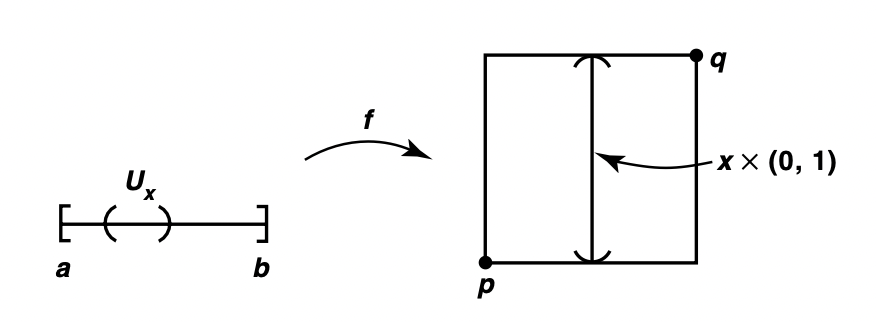
\includegraphics[width=.8\textwidth]{../images/Topology/5.png}
\label{}
\end{figure}

Choose for each \(x\in I\) a rational number \(q_x\in U_x\). Since the sets \(U_x\) are disjoint, the
map \(x\to q_x\) is an injective mapping of \(I\) into \(\Q\). This contradicts the fact that the
interval \(I\) is uncountable
\end{examplle}

\subsection{Compact Spaces}
\label{sec:org57e35eb}
\begin{definition}[]
A collection \(\cala\) of subsets of a space \(X\) is said to \textbf{cover} \(X\), or to be a \textbf{covering}
of \(X\), if \(\bigcup\cala=X\). It is called an \textbf{open covering} of \(X\) if its elements are open subsets of \(X\)
\end{definition}

\index{compact}
\begin{definition}[]
A space \(X\) is said to be \textbf{compact} if every open covering \(\cala\) of \(X\) contains a finite
subcollection that also covers \(X\).
\end{definition}

If \(Y\) is a subspace of \(X\), a collection \(\cala\) of subsets of \(X\) is said to \textbf{cover} \(Y\) if
the union of its elements \emph{contains} \(Y\)

\begin{lemma}[]
Let \(Y\) be a subspace of \(X\). Then \(Y\) is compact iff every covering of \(Y\) by sets open
in \(X\) contains a finite subcollection covering \(Y\).
\end{lemma}

\begin{proof}
If \(Y\) is compact and \(\cala=\{A_\alpha\}_{\alpha\in J}\) is a covering of \(Y\) by sets open in \(X\), then the
collection
\begin{equation*}
\{A_\alpha\cap Y\mid \alpha\in J\}
\end{equation*}
is a covering of \(Y\) by sets open in \(Y\); hence a finite subcollection
\begin{equation*}
\{A_{\alpha_1}\cap Y,\dots,A_{\alpha_n}\cap Y\}
\end{equation*}
covers \(Y\)

Conversely. Let \(\cala'=\{A'_\alpha\}\) be a covering of \(Y\) by sets open in \(Y\). For each
\(\alpha\), \(A_\alpha'=A_\alpha\cap Y\) for some \(A_\alpha\) open in \(X\). The
collection \(\{A_\alpha\}\) is a covering of \(Y\) by sets open in \(X\).
\end{proof}

\begin{theorem}[]
\label{thm26.2}
Every closed subspace of a compact space is compact
\end{theorem}

\begin{proof}
Let \(Y\) be a closed subspace of the compact space \(X\). Given a covering \(\cala\) of \(Y\) by
sets open in \(X\), let
\begin{equation*}
\calb=\cala\cup\{X-Y\}
\end{equation*}
Some finite subcollection of \(\calb\) covers \(X\).
\end{proof}

\begin{theorem}[]
\label{thm26.3}
Every compact subspace of a Hausdorff space is closed.
\end{theorem}

\begin{proof}
Let \(Y\) be a compact subspace of the Hausdorff space \(X\). We shall prove \(X-Y\) is open

Let \(x_0\) be a point of \(X-Y\). We show there is a neighborhood of \(x_0\) that is disjoint
from \(Y\). For each point \(y\) of \(Y\), choose disjoint neighborhoods \(U_y\) and \(V_y\) of
the points \(x_0\) and \(y\). The collection \(\{V_y\mid y\in Y\}\) is a covering of \(Y\) by sets open
in \(Y\); therefore, \(V_{y_1},\dots,V_{y_n}\) covers \(Y\). The open set
\begin{equation*}
V=Y_{y_1}\cup\dots\cup V_{y_n}
\end{equation*}
contains \(Y\), and its disjoint from the open set
\begin{equation*}
U=U_{y_1}\cap\dots\cap U_{y_n}
\end{equation*}
\end{proof}

\begin{lemma}[]
\label{lemma26.4}
if \(Y\) is a compact subspace of the Hausdorff space \(X\) and \(x_0\) is not in \(Y\), then
there exist disjoint open sets \(U\) and \(V\) of \(X\) containing \(x_0\) and \(Y\) respectively
\end{lemma}

\begin{examplle}[]
Once we prove that the interval \([a,b]\) in \(\R\) is compact, it follows from Theorem
\ref{thm26.2} that any closed subspace of \([a,b]\) is compact. On the other hand, it follows from
Theorem \ref{thm26.3} that the intervals \((a,b]\) and \((a,b)\) in \(\R\) cannot be compact since
they are not closed in Hausdorff space \(\R\).
\end{examplle}

\begin{theorem}[]
The image of a compact space under a continuous map is compact
\end{theorem}

\begin{theorem}[]
Let \(f:X\to Y\) be a bijectiive continuous function. If \(X\) is compact and \(Y\) is Hausdorff,
then \(f\) is homeomorphism
\end{theorem}

\begin{proof}
We shall prove that images of closed sets of \(X\) under \(f\) are closed in \(Y\). If \(A\) is
closed in \(X\), then \(A\) is compact, by Theorem \ref{thm26.2}. Therefore \(f(A)\) is compact.
Since \(Y\) is Hausdorff, \(f(A)\) is closed in \(Y\) by Theorem \ref{thm26.3}
\end{proof}

\begin{theorem}[]
The product of finitely many compact spaces is compact
\end{theorem}

\begin{proof}
We shall prove that the product of two compact spaces is compact;

Suppose we are given spaces \(X\) and \(Y\), with \(Y\) compact. Suppose that \(x_0\) is a point
of \(X\), and \(N\) is an open set of \(X\times Y\) containing \(x_0\times Y\). We prove the following
\begin{quoting}
There is a neighborhood \(W\) of \(x_0\) in \(X\) s.t. \(N\) contains the entire set \(W\times Y\)
\end{quoting}

The set \(W\times Y\) is often called a \textbf{tube} about \(x_0\times Y\)

First let's cover \(x_0\times Y\) by basis elements \(U\times V\) (for the topology of \(X\times Y\)), lying
in \(N\). The space \(x_0\times Y\)  is compact, being homeomorphic to \(Y\). Therefore, we can
cover \(x_0\times Y\) by finitely many such basis elements
\begin{equation*}
U_1\times V_1,\dots,U_n\times V_n
\end{equation*}
(We assume that each of the basis elements \(U_i\times V_i\)) actually intersects \(x_0\times Y\). Define
\begin{equation*}
W=U_1\cap\dots\cap U_n
\end{equation*}
\(W\) is open and it contains \(x_0\) because each set \(U_i\times V_i\) intersects \(x_0\times Y\).

We assert that the sets \(U_i\times V_i\), which were chosen to cover the slice \(x_0\times Y\), actually
cover the tube \(W\times Y\). Let \(x\times y\in W\times Y\). Consider the point \(x_0\times y\) of the
slice \(x_0\times Y\) having the same \(y\)-coordinate as this point. Now \(x_0\times y\in U_i\times V_i\) for
some \(i\), so that \(y\in V_i\). But \(x\in U_j\) for every \(j\). Therefore we
have a\(x\times y\in U_i\times V_i\) as desired

\begin{figure}[htbp]
\centering
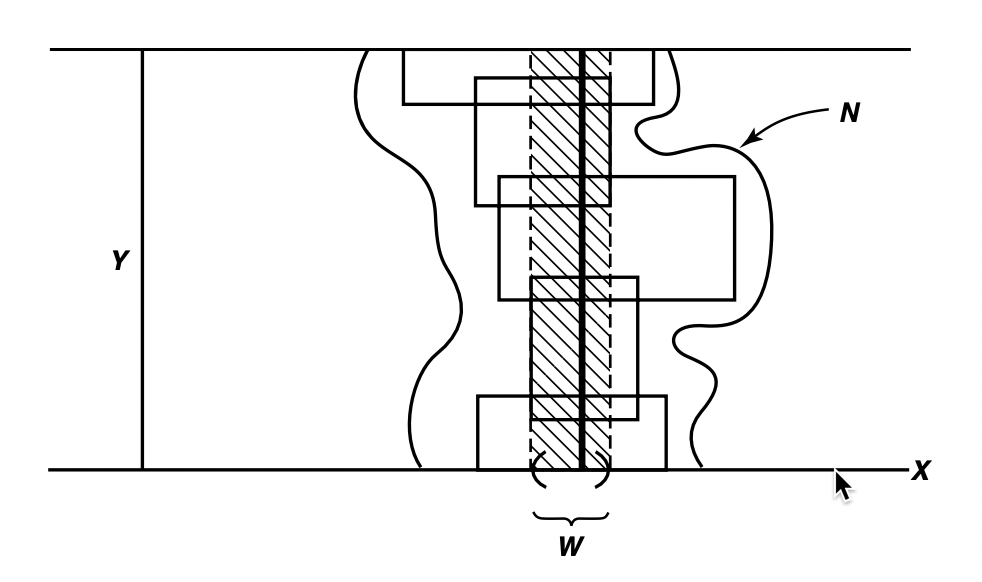
\includegraphics[width=.7\textwidth]{../images/Topology/6.png}
\label{}
\end{figure}

Now we prove the theorem. Let \(X\) and \(Y\) be compact spaces. Let \(\cala\) be an open covering
of \(X\times Y\). Given \(x_0\in X\), the slice \(x_0\times Y\) is compact and may therefore be covered by
finitely many elements \(A_1,\dots,A_m\in\cala\). \(N=A_1\cup\dots\cup A_m\) is an open set containing \(x_0\times Y\).

The open set \(N\) contains a tube \(W\times Y\) about \(x_0\times Y\) where \(W\) is open in \(X\).
Then \(W\times Y\) is covered by finitely many elements \(A_1,\dots,A_m\in\cala\).

Thus for each \(x\in X\), we can choose a neighborhood \(W_x\) of \(x\) s.t. the tube \(W_x\times Y\) can
be covered by finitely many elements of \(\cala\). The collection of all the neighborhoods \(W_x\) is
an open covering of \(X\); therefore by compactness of \(X\), there exists a finite subcollection
\begin{equation*}
\{W_1,\dots,W_k\}
\end{equation*}
covering \(X\). The union of the tubes
\begin{equation*}
W_1\times Y,\dots,W_k\times Y
\end{equation*}
is all of \(X\times Y\); since each may be covered by finitely many elements of \(\cala\).
\end{proof}

\begin{lemma}[The tube lemma]
\label{lemma26.8}
Consider the product space \(X\times Y\), where \(Y\) is compact. If \(N\) is an open set
of \(X\times Y\) containing the slice \(x_0\times Y\) of \(X\times Y\), then \(N\) contains some tube \(W\times Y\)
about \(x_0\times Y\) where \(W\) is a neighborhood of \(x_0\) in \(X\).
\end{lemma}

\begin{examplle}[]
The tube lemma is not true if \(Y\) is not compact. For example, let \(Y\) be the \(y\)-axis
in \(\R^2\), and
\begin{equation*}
N=\left\{x\times y\mid \abs{x}<\frac{1}{y^2+1}\right\}
\end{equation*}
Then \(N\) is an open set containing the set \(0\times \R\), but it contains no tube about \(0\times\R\)
\begin{figure}[htbp]
\centering
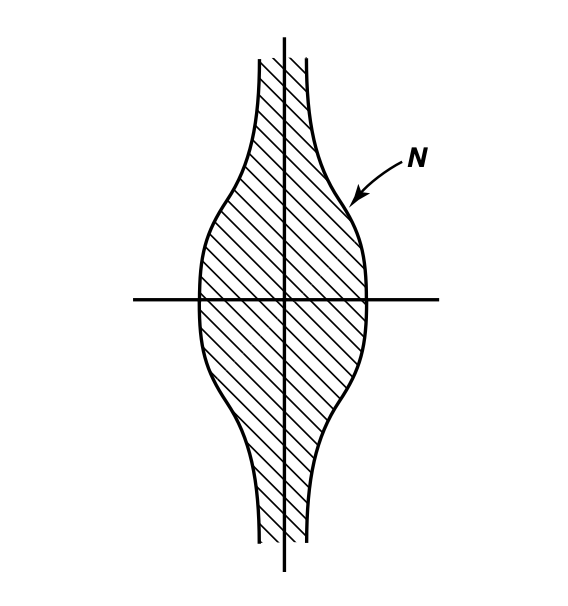
\includegraphics[width=.4\textwidth]{../images/Topology/7.png}
\label{}
\end{figure}
\end{examplle}

\begin{definition}[]
A collection \(\calc\)  of subsets of \(X\) is said to have the \textbf{finite intersection property} if for
every finite subcollection
\begin{equation*}
\{C_1,\dots,C_n\}
\end{equation*}
of \(\calc\), the intersection \(C_1\cap\dots\cap C_n\) is nonempty
\end{definition}

\begin{theorem}[]
\label{thm26.9}
Let \(X\) be a topological space. Then \(X\) is compact iff for every collection \(\calc\) of closed
sets in \(X\) having the finite intersection property, the intersection \(\bigcap_{C\in\calc}C\) is nonempty
\end{theorem}

\begin{proof}
Given a collection \(\cala\) of subsets of \(X\), let
\begin{equation*}
\calc=\{X-A\mid A\in\cala\}
\end{equation*}
Then the following holds
\begin{enumerate}
\item \(\cala\) is a collection of open sets iff \(\calc\) is a collection of closed sets
\item The collection \(\cala\) covers \(X\) iff the intersection \(\bigcap_{C\in\calc}C\) is empty
\item The finite subcollection \(\{A_1,\dots,A_n\}\) of \(\cala\) covers \(X\) iff \(\bigcap C_i\) is empty
\end{enumerate}


Take the contrapositive of the theorem: given any collection \(\cala\) of open sets, if no finite
subcollection of \(\cala\) covers \(X\), then \(\cala\) does not cover \(X\), which is equivalent to:
given any collection \(\calc\) of closed sets, if every finite intersection of elements of \(\calc\) is
nonempty, then the intersection of all the elements of \(\calc\) is nonempty
\end{proof}

A special case of this theorem occurs when we have a \textbf{nested sequence} \(C_1\supset\dots\supset C_n\supset\dots\) of closed
sets in a compact space \(X\). If each of the sets \(C_n\) is nonempty, then the
collection \(\calc=\{C_n\}_{n\in\Z_+}\) automatically has the finite intersection property. Then the
intersection
\begin{equation*}
\bigcup_{n\in\Z_+}C_n
\end{equation*}
is nonempty

\begin{exercise}
\label{ex26.1}
\begin{enumerate}
\item Let \(\calt\) and \(\calt'\) be two topologies on the set \(X\); suppose that \(\calt'\supset\calt\). what does
compactness of \(X\) under one of these topologies imply about compactness under the other
\item show that if \(X\) is compact Hausdorff under both \(\calt\) and \(\calt'\), then either \(\calt=\calt'\) or
they are not comparable
\end{enumerate}
\end{exercise}

\begin{proof}
\begin{enumerate}
\item if \((X,\calt')\) is compact then so is \((X,\calt)\)
\item Suppose one is finer than the other. Then the identity mapping from the finer one to the
coarser one is a continuous and bijectiive function that maps a compact space to a Hausdorff
space. Therefore it is a homeomorphism and the topologies are the same
\end{enumerate}
\end{proof}

\begin{exercise}
\label{ex26.2}
\begin{enumerate}
\item Show that in the finite complement topology on \(\R\), every subspace is compact
\item If \(\R\) has the topology consisting of all sets \(A\) s.t. \(\R-A\) is either countable or all
of \(\R\), is \([0,1]\) a compact subspace?
\end{enumerate}
\end{exercise}

\begin{proof}
\begin{enumerate}
\item Given any covering \(\cala\) of the subspace, \(\R-\bigcup\cala\) is finite and we can choose the set one by one
\item No. Let \(A_n=[0,1]-\{1/n,1/(n+1),\dots\}\)
\end{enumerate}
\end{proof}

\begin{exercise}
\label{ex26.3}
Show that a finite union of compact subspaces of \(X\) is compact
\end{exercise}

\begin{exercise}
\label{ex26.4}
Show that every compact subspace of a metric space is bounded in that metric and is closed. Find
a metric space where not every closed bounded subspace is compact. Find a metric space in which
not every closed bounded subspace is compact.
\end{exercise}

\begin{proof}
If it were not bounded, then for any ball there would be a point outside it, and while the union
of all these ball does cover the whole space, there is no finite subcovering for the subspace
\end{proof}

\begin{exercise}
Show that if \(f:X\to Y\) is continuous, where \(X\) is compact and \(Y\) is Hausdorff, then \(f\)
is a closed map (that is, \(f\) carries closed sets to closed sets)
\end{exercise}

\subsection{Compact Subspaces of the Real Line}
\label{sec:orga0c10a8}
\begin{theorem}[]
Let \(X\) be a simply ordered set having the least upper bound property. In the order topology,
each closed interval in \(X\) is compact
\end{theorem}

\begin{proof}
\emph{Step 1}. Given \(a<b\), let \(\cala\) be a covering of \([a,b]\) by sets open in \([a,b]\) in the
subspace topology (which is the same as the order topology). First we prove the following
\begin{quoting}
If \(x\in[a,b]\) different from \(b\), then there is a point \(y>x\) of \([a,b]\) s.t. the interval \([x,y]\) can
be covered by at most two elements of \(\cala\).
\end{quoting}

If \(x\) has an immediate successor in \(X\), let \(y\) be this immediate successor.
Then \([x,y]\) has two points \(x,y\). If \(x\) has no immediate successor in \(X\), choose an
element \(A\in\cala\) containing \(x\). Because \(x\neq b\) and \(A\) is open, \(A\) contains an interval
of the form \([x,c)\) for some \(c\in[a,b]\). Choose a point \(y\in(x,c)\), then \([x,y]\) can be
covered by \(A\).

\emph{Step 2}. Let \(C\) be the set of all points \(y>a\) of \([a,b]\) s.t. the interval \([a,y]\) can
be covered by finitely many elements of \(\cala\). Applying Step 1 to the case \(x=a\), we see that
there exists at least one such \(y\), so \(C\) is not empty. Let \(c\) be the least upper bound
of the set \(C\); then \(a<c\le b\)

\emph{Step 3}. We show that \(c\in C\). Choose an element \(A\in\cala\) containing \(c\). Since \(A\) is open,
it contains an interval of the form \((d,c]\) for some \(d\in[a,b]\). It \(c\not\in C\), there must
be a point \(z\in C\) lying in the interval \((d,c)\), because otherwise \(d\)would be a smaller
upper bound on \(C\) than \(c\). Since \(z\in C\), the interval \([a,z]\) can be covered by
finitely many, say \(n\), elements of \(\cala\). Now \([z,c]\) lies in the single elements \(A\)
of \(\cala\), hence \([a,c]=[a,z]\cup[z,c]\) can be covered by \(n+1\) elements of \(\cala\). Thus \(c\in C\)

\emph{Step 4}. Finally we show that \(c=b\). Suppose \(c<b\), applying Step 1 to the case \(x=c\) we
conclude that there exists a point \(y>c\) of \([a,b]\) s.t. the interval \([c,y]\) can be
covered by finitely many elements of \(\cala\).  By Step 3, \([a,y]\) can be covered by finitely many
elements of \(\cala\). This means that \(y\in C\), a contradiction
\end{proof}

\begin{corollary}[]
Every closed interval in \(\R\) is compact
\end{corollary}

\begin{theorem}[]
A subspace \(A\) of \(\R^n\) is compact iff it is closed and its bounded in the euclidean
metric \(d\) or the square metric \(\rho\)
\end{theorem}

\begin{proof}
It will suffice to consider only the metric \(\rho\); the inequalities
\begin{equation*}
\rho(x,y)\le d(x,y)\le\sqrt{n}\rho(x,y)
\end{equation*}
imply that \(A\)is bounded under \(d\) iff it is bounded under \(\rho\)

Suppose that \(A\) is compact. Then by Theorem \ref{thm26.3} it is closed. Consider the collection
of open sets
\begin{equation*}
\{B_\rho(\textbf{0},m)\mid m\in\Z_+\}
\end{equation*}
whose union is all of \(\R^+\). Some finite subcollection covers \(A\). It follows
that \(A\subset B_\rho(\textbf{0},M)\) for some \(M\). Therefore, for any two
points \(x,y\in A\), \(\rho(x,y)\le 2M\)

Conversely, suppose that \(A\) is closed and bounded under \(\rho\); suppose \(\rho(x,y)\le N\) for
every \(x,y\in A\). Choose a point \(x_0\in A\) and let \(\rho(x_0,\textbf{0})=b\). The triangle
inequality implies that \(\rho(x,\textbf{0})\le N+b\) for every \(x\in A\). If \(P=N+b\), then \(A\) is
a subset of the cube \([-P,P]^n\) , which is compact. Being closed, \(A\) is also compact.
\end{proof}

\begin{theorem}[Extreme value theorem]
Let \(f:X\to Y\) be continuous, where \(Y\) is an ordered set in the order topology. If \(X\) is
compact, then there exist points \(c\) and \(d\) in \(X\) s.t. \(f(c)\le f(x)\le f(d)\) for
every \(x\in X\).
\end{theorem}

\begin{proof}
Since \(f\) is continuous and \(X\) is compact, the set \(A=f(X)\) is compact. We show that \(A\)
has a largest element \(M\) and a smallest element \(x\).

If \(A\) has no largest element, then the collection
\begin{equation*}
\{(-\infty,a)\mid a\in A\}
\end{equation*}
forms an open covering of \(A\). Since \(A\) is compact, some finite subcollection
\begin{equation*}
\{(-\infty,a_1),\dots,(-\infty,a_n)\}
\end{equation*}
covers \(A\). If \(a_i=\max\{a_1,\dots,a_n\}\) , then \(a_i\) belongs to none of these sets, contrary to
the fact that they cover \(A\)
\end{proof}

\begin{definition}[]
Let \((X,d)\) be a metric space; let \(A\) be a nonempty subset of \(X\) . For each \(x\in X\) we
define the \textbf{distance from \(x\) to \(A\)} by the equation
\begin{equation*}
d(x,A)=\inf\{d(x,a)\mid a\in A\}
\end{equation*}
\end{definition}

Fix \(A\), then the function \(d(x,A)\) is a continuous function of \(x\): Given \(x,y\in X\), one
has the inequalities
\begin{equation*}
d(x,A)\le d(x,a)\le d(x,y)+d(y,a)
\end{equation*}
for each \(a\in A\). It follows that
\begin{equation*}
d(x,A)-d(x,y)\le\inf d(y,a)=d(y,A)
\end{equation*}
so that
\begin{equation*}
d(x,A)-d(y,A)\le d(x,y)
\end{equation*}
Continuity of the function \(d(x,A)\) follows

\begin{lemma}[The Lebesgue number lemma]
Let \(\cala\) be an open covering of the metric space \((X,d)\). If \(X\) is compact, there is
a \(\delta>0\) s.t. for each subset of \(X\) having diameter less than \(\delta\), there exists an element
of \(\cala\) containing it
\end{lemma}

The number \(\delta\) is called a \textbf{Lebesgue number} for the covering \(\cala\).

\begin{proof}
Let \(\cala\) be an open covering of \(X\). If \(X\in\cala\), then any positive number is a Lebesgue number
for \(\cala\). So assume \(X\) is not an element of \(\cala\)

Choose a finite subcollection \(\{A_1,\dots,A_n\}\) of \(\cala\) that covers \(X\). For each \(i\),
set \(C_i=X-A_i\), and define \(f:X\to\R\) by letting \(f(x)\) be the average of the
numbers \(d(x,C_i)\). That is,
\begin{equation*}
f(x)=\frac{1}{n}\sum_{i=1}^nd(x,C_i)
\end{equation*}
We show that \(f(x)>0\) for all \(x\). Given \(x\in X\), choose \(i\) so that \(x\in A_i\). Then
choose \(\epsilon\) so the \(\epsilon\)-neighborhood of \(x\) lies in \(A_i\). Then \(d(x,C_i)\ge\epsilon\), so that \(f(x)\ge\epsilon/n\).

Since \(f\) is continuous, it has a minimum value \(\delta\); we show that \(\delta\) is our required Lebesgue
number. Let \(B\) the be a subset of \(X\) of diameter less than \(\delta\). Choose a point \(x_0\in B\);
then \(B\) lies in the \(\delta\)-neighborhood of \(x_0\). Now
\begin{equation*}
\delta\le f(x_0)\le d(x_0,C_m)
\end{equation*}
where \(d(x_0,C_m)=\max\{d(x_0,C_i)\}\). Then the \(\delta\)-neighborhood of \(x_0\) is contained in the
element \(A_m=X-C_m\) of the covering \(\cala\).
\end{proof}

\begin{definition}[]
A function \(f\) from the metric space \((X,d_X)\) to the metric space \((Y,d_Y)\) is said to be
\textbf{uniformly continuous} if given \(\epsilon>0\) there is a \(\delta>0\) s.t. for every pair of points \(x_0,x_1\)
of \(X\),
\begin{equation*}
d_X(x_0,x_1)<\delta\Longrightarrow d_Y(f(x_0),f(x_1))<\epsilon
\end{equation*}
\end{definition}

\begin{theorem}[Uniform continuity theorem]
Let \(f:X\to Y\) be a continuous map of the compact metric space \((X,d_X)\) to the metric
space \((Y,d_Y)\). Then \(f\) is uniformly continuous
\end{theorem}

\begin{proof}
Given \(\epsilon>0\), take the open covering of \(Y\) by balls \(B(y,\epsilon/2)\) of radius \(\epsilon/2\). Let \(\cala\)
be the open covering of \(X\) by the inverse images of these balls under \(f\). Choose \(\delta\) to be a
Lebesgue number for the covering \(\cala\). Then if \(x_1,x_2\in X\) s.t. \(d_X(x_1,x_2)<\delta\) the two-point
set \(\{x_1,x_2\}\) has diameter less than \(\delta\), so that its image \(\{f(x_1),f(x_2)\}\) lies in some
ball \(B(y,\epsilon/2)\). Then \(d_Y(f(x_1),f(x_2))<\epsilon\) as desired.
\end{proof}

\begin{definition}[]
If \(X\) is a space, a point \(x\in X\) is said to be an \textbf{isolated point} of \(X\) if the one-point
set \(\{x\}\) is open in \(X\)
\end{definition}

\begin{theorem}[]
Let \(X\) be a nonempty compact Hausdorff space. If \(X\) has no isolated points, then \(X\) is uncountable
\end{theorem}

\begin{proof}
\emph{Step 1}. We show first that given any nonempty open set \(U\) of \(X\) and any point \(x\in X\),
there exists a nonempty open set \(V\) contained in \(U\) s.t. \(x\not\in\barVV\)

Choose a point \(y\in U\) different from \(x\); this is possible if \(x\in U\) since \(x\) is not an
isolated point of \(X\) and it is possible if \(x\not\in U\) since \(U\) is nonempty. Now choose
disjoint open sets \(x\in W_1\) and \(y\in W_2\). Then \(V=W_2\cap U\) is the desired open set.

\begin{figure}[htbp]
\centering
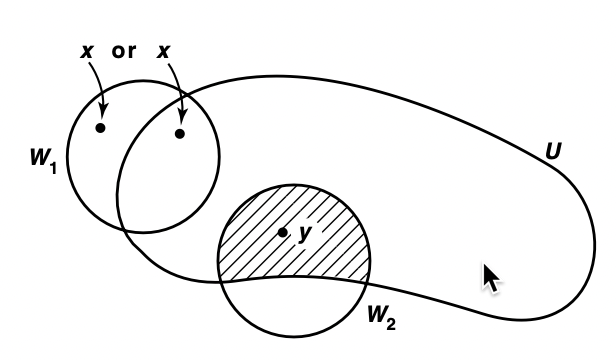
\includegraphics[width=.7\textwidth]{../images/Topology/8.png}
\label{}
\end{figure}

\emph{Step 2}. We show that given \(f:\Z_+\to X\) the function \(f\) is not surjective. It follows
that \(X\) is uncountable

Let \(x_n=f(n)\). Apply Step 1 to the nonempty open set \(U=X\) to choose a nonempty open
set \(V_1\subset X\) s.t. \(x_1\not\in\barVV_1\). In general, given \(V_{n-1}\) open and nonempty,
choose \(V_n\) to be a nonempty open set s.t. \(V_n\subset V_{n-1}\) and \(\barVV_n\) doesn't
contain \(x_n\). Consider the nested sequence
\begin{equation*}
\barVV_1\supset \barVV_2\supset\cdots
\end{equation*}
of nonempty closed sets of \(X\). Because \(X\) is compact, there is a point \(x\in\bigcup\barVV_n\), by
Theorem \ref{thm26.9}. Now \(x\neq x_n\) for any \(n\).
\end{proof}

\begin{corollary}[]
Every closed interval in \(\R\) is uncountable
\end{corollary}

\begin{exercise}
\label{ex27.2}
Let \(X\) be a metric space with metric \(d\); let \(A\subset X\) be nonempty
\begin{enumerate}
\item Show that \(d(x,A)=0\) iff \(x\in\barA\)
\item Show that if \(A\) is compact, \(d(x,A)=d(x,a)\) for some \(a\in A\)
\end{enumerate}
\end{exercise}

\begin{proof}
\begin{enumerate}
\setcounter{enumi}{1}
\item 
\end{enumerate}
\end{proof}
\end{document}
